%%%%%%%%%%%%%%%%%%%%%%%%%%%%%%%%%%%%%%%%%
% Thesis 
% LaTeX Template
% Version 1.3 (21/12/12)
%
% This template has been downloaded from:
% http://www.latextemplates.com
%
% Original authors:
% Steven Gunn 
% http://users.ecs.soton.ac.uk/srg/softwaretools/document/templates/
% and
% Sunil Patel
% http://www.sunilpatel.co.uk/thesis-template/
%
% License:
% CC BY-NC-SA 3.0 (http://creativecommons.org/licenses/by-nc-sa/3.0/)
%
% Note:
% Make sure to edit document variables in the Thesis.cls file
%
%%%%%%%%%%%%%%%%%%%%%%%%%%%%%%%%%%%%%%%%%

%----------------------------------------------------------------------------------------
%	PACKAGES AND OTHER DOCUMENT CONFIGURATIONS
%----------------------------------------------------------------------------------------

\documentclass[11pt, a4paper, oneside]{Thesis} % Paper size, default font size and one-sided paper

\graphicspath{{./Pictures/}} % Specifies the directory where pictures are stored

\usepackage[comma]{natbib}
%\usepackage[comma, sort&compress]{natbib} % Use the natbib reference package - read up on this to edit the reference style; if you want text (e.g. Smith et al., 2012) for the in-text references (instead of numbers), remove 'numbers'
\usepackage[utf8]{inputenc}
\usepackage{float}
\usepackage{fancyvrb}
\usepackage[linesnumbered,ruled]{algorithm2e}
\usepackage{amsmath}
\usepackage{lingmacros}
\usepackage{rotating}
\hypersetup{urlcolor=black, colorlinks=true} % Colors hyperlinks in blue - change to black if annoying
\title{\ttitle} % Defines the thesis title - don't touch this

\begin{document}

\frontmatter % Use roman page numbering style (i, ii, iii, iv...) for the pre-content pages

\setstretch{1.3} % Line spacing of 1.3

% Define the page headers using the FancyHdr package and set up for one-sided printing
\fancyhead{} % Clears all page headers and footers
\rhead{\thepage} % Sets the right side header to show the page number
\lhead{} % Clears the left side page header

\pagestyle{fancy} % Finally, use the "fancy" page style to implement the FancyHdr headers

\newcommand{\HRule}{\rule{\linewidth}{0.5mm}} % New command to make the lines in the title page

% PDF meta-data
\hypersetup{pdftitle={\ttitle}}
\hypersetup{pdfsubject=\subjectname}
\hypersetup{pdfauthor=\authornames}
\hypersetup{pdfkeywords=\keywordnames}

%----------------------------------------------------------------------------------------
%	TITLE PAGE
%----------------------------------------------------------------------------------------

\begin{titlepage}
\begin{center}

\textsc{\LARGE \univname}\\[0.1cm]
\textsc{Faculteit der Natuurwetenschappen, Wiskunde en Informatica} \\[1cm] % University name
\textsc{\Large MSc Thesis}\\[0.5cm] % Thesis type

\HRule \\[0.4cm] % Horizontal line
{\huge \bfseries \ttitle}\\[0cm] % Thesis title
\HRule \\[1.5cm] % Horizontal line

\begin{minipage}{0.4\textwidth}
\begin{flushleft} \large
\emph{Author:}\\
\authornames % Author name - remove the \href bracket to remove the link
\end{flushleft}
\end{minipage}
\begin{minipage}{0.4\textwidth}
\begin{flushright} \large
\emph{Supervisor:} \\
\supname % Supervisor name - remove the \href bracket to remove the link  
\end{flushright}
\end{minipage}\\[3cm]
 
\large \textit{A thesis submitted in fulfillment of the requirements\\ for the degree of \degreename}\\[0.3cm] % University requirement text
\textit{in the}\\[0.4cm]
\deptname\\[2cm] % Research group name and department name

{\large \today}\\[2cm] % Date
\includegraphics[height=3cm]{uva-logo} % University/department logo - uncomment to place it

\vfill
\end{center}

\end{titlepage}

%----------------------------------------------------------------------------------------
%	DECLARATION PAGE
%	Your institution may give you a different text to place here
%----------------------------------------------------------------------------------------

%\Declaration{

%\addtocontents{toc}{\vspace{1em}} % Add a gap in the Contents, for aesthetics

%I, \authornames, declare that this thesis titled, '\ttitle' and the work presented in it are my own. I confirm that:

%\begin{itemize} 
%\item[\tiny{$\blacksquare$}] This work was done wholly or mainly while in candidature for a research degree at this University.
%\item[\tiny{$\blacksquare$}] Where any part of this thesis has previously been submitted for a degree or any other qualification at this University or any other institution, this has been clearly stated.
%\item[\tiny{$\blacksquare$}] Where I have consulted the published work of others, this is always clearly attributed.
%\item[\tiny{$\blacksquare$}] Where I have quoted from the work of others, the source is always given. With the exception of such quotations, this thesis is entirely my own work.
%\item[\tiny{$\blacksquare$}] I have acknowledged all main sources of help.
%\item[\tiny{$\blacksquare$}] Where the thesis is based on work done by myself jointly with others, I have made clear exactly what was done by others and what I have contributed myself.\\
%\end{itemize}
 
%Signed:\\
%\rule[1em]{25em}{0.5pt} % This prints a line for the signature
 
%Date:\\
%\rule[1em]{25em}{0.5pt} % This prints a line to write the date
%}

%\clearpage % Start a new page

%----------------------------------------------------------------------------------------
%	QUOTATION PAGE
%----------------------------------------------------------------------------------------

\pagestyle{empty} % No headers or footers for the following pages

\null\vfill % Add some space to move the quote down the page a bit

\textit{``Non sono programmato per l'umorismo. E, comunque, non di primo mattino!"}

\small
``I'm not programmed for humour. Not early in the morning, anyway!"
\normalsize
\begin{flushright}
Uno, PKNA \#0
\end{flushright}

\vfill\vfill\vfill\vfill\vfill\vfill\null % Add some space at the bottom to position the quote just right

\clearpage % Start a new page

%----------------------------------------------------------------------------------------
%	ABSTRACT PAGE
%----------------------------------------------------------------------------------------

\addtotoc{Abstract} % Add the "Abstract" page entry to the Contents

\abstract{\addtocontents{toc}{\vspace{1em}} % Add a gap in the Contents, for aesthetics

As human-computer interaction technologies advance, the gap between the language of computer systems and the one of their users reduces, thanks to the inclusion of typical elements of human-human interaction such as visuals, haptics or natural language. In this sense, developments in the field of \textbf{dialogue systems} are central. In this thesis we address some issues that most modern dialogue systems are still struggling with.

A basic fact about human-human dialogue is that there is often more than one way of talking about any domain. Often language \textbf{understanding} and production abilities of dialogue systems are limited to a static vocabulary of predefined sentences. We propose a system that is able to perform flexible meaning matching to grasp the meaning of sentences that were never encountered before.

Secondly, linguistic abilities in humans evolve, as new interactions are performed, and new expressions are learned. Our system \textbf{learns} new elements of the language from successful interactions with the user.

Lastly, human dialogue is a social activity, in that it involves continuous attention of the dialogue partners (DPs) to each other's understanding. The act of establishing mutual knowledge among the DPs is called \textbf{grounding}, and it's still a topic of research in dialogue systems. Our system is able to detect potential misinterpretation of user utterances, interact with him to clarify their meaning, and learn from this interaction.
}

\clearpage % Start a new page

%----------------------------------------------------------------------------------------
%	ACKNOWLEDGEMENTS
%----------------------------------------------------------------------------------------

%\setstretch{1.3} % Reset the line-spacing to 1.3 for body text (if it has changed)

%\acknowledgements{\addtocontents{toc}{\vspace{1em}} % Add a gap in the Contents, for aesthetics

%The acknowledgements and the people to thank go here\ldots

% Other people to acknowledge
% - The guy who created this template: http://www.latextemplates.com/template/masters-doctoral-thesis
%}
%\clearpage % Start a new page

%----------------------------------------------------------------------------------------
%	LIST OF CONTENTS/FIGURES/TABLES PAGES
%----------------------------------------------------------------------------------------

\pagestyle{fancy} % The page style headers have been "empty" all this time, now use the "fancy" headers as defined before to bring them back

\lhead{\emph{Contents}} % Set the left side page header to "Contents"
\tableofcontents % Write out the Table of Contents

\lhead{\emph{List of Figures}} % Set the left side page header to "List of Figures"
\listoffigures % Write out the List of Figures

%\lhead{\emph{List of Tables}} % Set the left side page header to "List of Tables"
%\listoftables % Write out the List of Tables

%----------------------------------------------------------------------------------------
%	ABBREVIATIONS
%----------------------------------------------------------------------------------------

\clearpage % Start a new page

\setstretch{1.5} % Set the line spacing to 1.5, this makes the following tables easier to read

\lhead{\emph{Abbreviations}} % Set the left side page header to "Abbreviations"
\listofsymbols{ll} % Include a list of Abbreviations (a table of two columns)
{
\textbf{AI} & \textbf{A}rtificial \textbf{I}ntelligence \\
\textbf{ASR} & \textbf{A}utomatic \textbf{S}peech \textbf{R}ecognition \\
\textbf{CA} & \textbf{C}onversational \textbf{A}gent \\
\textbf{DM} & \textbf{D}ialogue \textbf{M}anager \\
\textbf{DP} & \textbf{D}ialogue \textbf{P}artner \\
\textbf{ISU} & \textbf{I}nformation \textbf{S}tate \textbf{U}pdate \\
\textbf{LU} & \textbf{L}anguage \textbf{U}nit \\
\textbf{ML} & \textbf{M}achine \textbf{L}earning \\
\textbf{MT} & \textbf{M}achine \textbf{T}ranslation \\
\textbf{NLP} & \textbf{N}atural \textbf{L}anguage \textbf{P}rocessing \\
\textbf{SLU} & \textbf{S}poken \textbf{L}anguage \textbf{U}nderstanding \\
\textbf{TDM} & \textbf{T}RINDIKIT \textbf{D}ialogue \textbf{M}anager \\
\textbf{TTS} & \textbf{T}ext \textbf{T}o \textbf{S}peech \\
%\textbf{Acronym} & \textbf{W}hat (it) \textbf{S}tands \textbf{F}or \\
}

%----------------------------------------------------------------------------------------
%	SYMBOLS
%----------------------------------------------------------------------------------------

\clearpage % Start a new page

\lhead{\emph{Symbols}} % Set the left side page header to "Symbols"

\listofnomenclature{lll} % Include a list of Symbols (a three column table)
{
$m$ & meaning \\
$c$ & chunk of text \\
$s$ & sentence \\
% Symbol & Name & Unit \\

& & \\ % Gap to separate the Roman symbols from the Greek

$\sigma$ & similarity score \\
$\sigma_m$ & Meaning Score \\
$\sigma_s$ & Sentence Score \\
$\sigma_c$ & Chunk Score \\
$\sigma_w$ & Word Score \\
$\tau$ & Word Score \\
% Symbol & Name & Unit \\
}

%----------------------------------------------------------------------------------------
%	DEDICATION
%----------------------------------------------------------------------------------------

%\setstretch{1.3} % Return the line spacing back to 1.3

%\pagestyle{empty} % Page style needs to be empty for this page

%\dedicatory{For/Dedicated to/To my\ldots} % Dedication text

%\addtocontents{toc}{\vspace{2em}} % Add a gap in the Contents, for aesthetics

%----------------------------------------------------------------------------------------
%	THESIS CONTENT - CHAPTERS
%----------------------------------------------------------------------------------------

\mainmatter % Begin numeric (1,2,3...) page numbering

\pagestyle{fancy} % Return the page headers back to the "fancy" style

% Include the chapters of the thesis as separate files from the Chapters folder
% Uncomment the lines as you write the chapters

% Chapter Template

\chapter{Introduction} % Main chapter title

\label{ch:Introduction} % Change X to a consecutive number; for referencing this chapter elsewhere, use \ref{ChapterX}

\lhead{\emph{Introduction}} % Change X to a consecutive number; this is for the header on each page - perhaps a shortened title

%----------------------------------------------------------------------------------------
%	INTRO TEXT
%----------------------------------------------------------------------------------------


The \textbf{user interface}, or human-computer interface, is the component of a computer system that provides a space of interaction between the human user and the resources offered by the machine; such a space defines a bridge language which human intentions can be translated into, to be converted into computational procedures for the machine; vice versa, the result of the computation is then presented to the user in the same language, which he or she is assumed to understand.

% cite Tanenbaum
In the early days of computing, the so-called \textbf{batch interfaces} were non-interactive: the user/programmer was supposed to feed the machine with a software, punched on cards using the \textit{machine's assembly language} directly, and retrieve the result of the computation printed on paper. The third and fourth generations of computing brought \textbf{text-based} interfaces for operating systems (UNIX, DOS, CP/M), that were later taken over by \textbf{Graphical User Interfaces} (GUI), moving the human-machine interaction on a new, visual language made of windows, icons and buttons. Recently, touch screen and camera devices allowed for the implementation of even more natural means of interaction based on \textbf{gestures} and physical actions.

From this brief spot on computing history, and in a way from common sense, we can draw the rather trivial, yet crucial, conclusion that the trend in user interfaces development is to \textbf{close the gap} between humans and machines by moving the needle of the interface languages from a machine-centered space towards the human language itself. To this respect, the studies on Natural Language Processing (NLP) assume a dramatically central role, as dramatically central is natural language in the interaction of humans with each other.

For this reason, the focus of this thesis work is the area of \textbf{dialogue systems}. A spoken dialogue system, or conversational agent (CA), allows humans and machines to interact through an intermediate language which is as close as possible to the \textbf{human language}, and through conversational episodes that implement as close as possible the human dialogue modalities.

%----------------------------------------------------------------------------------------
%	LEARNING TO TALK
%----------------------------------------------------------------------------------------

\section{Learning to talk}

One of the constituent features of humans' ability to speak is that such an ability doesn't come fully developed in children, but rather \textbf{grows} with time, influenced by the interaction of the subject with the outer world.
%~ One of the constituent features of humans' ability to speak is that such an ability is \textbf{not innate}, but is rather learned through interactions.

Ever since the power of computers grew enough to allow for intensive statistical analysis of significant amounts of data, \textbf{Machine Learning} approaches to Artificial Intelligence tasks got more and more prominent in the scene, often outperforming static methods (i.e. where the solution procedure for a task is explicitly coded by the programmer).
% Citation needed...
One of the clearest examples is the field of NLP itself, where the most important tasks, like parsing or machine translation, are dominated by Machine Learning methods based on corpora,
% Citation needed
meaning that, for instance, a Machine Translation system will first be trained on a corpus of aligned sentences. Statistical structures will be extracted from this corpus, like the most likely word-by-word alignment, and later be used to process new examples.

However, the task of learning through dialogue interactions comes with some \textbf{peculiar} challenges. First of all, humans learning to talk do not go through two separate phases of learning and processing, but rather improve their abilities episode by episode; as \cite{2095408} point out, this \textbf{incremental learning} structure is nowadays not implemented in state-of-the-art systems. Also, the nature of this incrementing learning is \textbf{not linear}, as the new information was stacked little by little on the existing one: new words and phrases can be described with concepts and linguistic structures that are already present in the learner's mind. Lastly, if we keep considering the way humans learn to talk, we realize that, as from a certain point, the language ceases to be a mere subject of learning, and \textbf{becomes the means} by which it is itself learned: the same linguistic structures that are used to express concepts and categories of the learner's experience, can also be used to describe themselves, as they become part of the same experience; we can observe a clear example of this process in any primary-school-level English class, where the teacher explains, by using English sentences, how English sentences are structured.

We can identify some \textbf{ideal features} we would like to have implemented into an automatic language learner:
\begin{itemize}
	\item Learning to produce or understand new surface forms, or \textbf{realizations}, for a given meaning -- eg. the sentence ``Bill eats an apple" for the action of Bill eating an apple.
	\item Learning to produce new \textbf{meanings} from the existing ones and their respective realizations -- eg. the concept of motor home, sharing the features of a house and a car.
	\item Learning a \textbf{``grammar" of conversation}, to place the correct utterance at each step of a conversational episode. -- eg. an appropriate answer to the utterance ``My name is Bill" can be ``Nice to meet you", whereas ``I like cookies" would not sound as much appropriate.
	%~ \item Learning to talk about its \textbf{meta} level, that is, the structures that control the production of utterances, like the syntax according to which new utterances are formed, or the ``grammar" of conversation of the previous point. 
\end{itemize}
Lastly, we can point out that when we talk of such things like \emph{realizations}, \emph{meanings} and \emph{episodes} we cannot provide exact, sharply bounded definitions, as it can be argued for \textbf{recursive and compositional} structures at any level of their interpretation. As an example, let's consider the sentence \enumsentence{I am pronouncing a sentence that contains two verbs and three nouns} The meaning of such a sentence describes structural elements of the sentence itself (which is the realization of the same meaning) and also the conversational episode that starts when the sentence is stated.

%----------------------------------------------------------------------------------------
%	THIS THESIS PROJECT
%----------------------------------------------------------------------------------------

\section{This thesis project} \label{ch:intro:project}

The aim of this thesis project is to design and implement language learning capabilities for an existing dialogue system, focusing on the \textbf{realization level}. That is, given a fixed list of meanings, the system should be able to classify every given sentence into its correct meaning. A client application has also been developed, that makes use of the dialogue system to solve a real user experience task.

Such an application is a voice-controlled music player, which has been named \textbf{\pname}. The task of such an application is to to get natural language input from the user and translate it into an appropriate corresponding behaviour. For example, when the input is ``Play Pictures at an exhibition", the system should start playing the famous suite by Modest Mussorgsky.

In this domain, each \textbf{meaning} corresponds to an action that the player can perform (e.g.\ play a song, jump to the next track, increase the volume, etc.), and is defined by a set of representative sentences, being its surface forms. For instance, the action of increasing the volume level can be defined by the following set of sentences:
\enumsentence{Increase the volume}
\enumsentence{Increase the volume level}
\enumsentence{Raise the volume}
\enumsentence{Increase the volume please}

The \textbf{task} for the application is, given an arbitrary input sentence and a context (the point of the conversational episode being realized), to reply appropriately, and perform the correct action, that is, \textbf{associate} that sentence with its correct meaning. Furthermore, the system should be able to \textbf{learn} new realizations for each meaning, as unknown sentences are given in input and processed.

Note that such processing might be more or less \textbf{semantically intensive}. As an example, it can be argued that, given the above definition of the action to increase the volume, matching \textit{``Raise the volume please"} is an easier task than classifying \textit{``Turn up the volume"}. This is because the first sentence can be seen as a mere, string-wise, fusion of the two existing examples \textit{``Raise the volume"} and \textit{``Increase the volume please"}, whereas the second one requires a model of \textit{``Turn up"} being a string that carries the same meaning as other strings like \textit{``Increase"} or \textit{``Raise"}.

Also, an unknown input sentence should be given a \textbf{confidence score} for each candidate meaning it is associated to, in order for the system to model the uncertainty in the classification of unknown examples. This is important because, depending on the degree of confidence of an interpretation, the system may change its interaction plans (e.g.\ asking the user for clarification).

Finally, the system should be able to narrow possible needs for \textbf{clarification} down to single sentence components, eventually asking the user for disambiguation as specifically as possible. This is to enforce the learning of small components that may appear again in further unknown examples.

This document is structured as follows. Chapter \ref{ch:rw} reviews the \textbf{related work} that has been previously done; chapter \ref{ch:arch} describes the \textbf{architecture} of the solution that has been developed; chapter \ref{ch:M2} delves into the \textbf{M2 algorithm}, which is the core of the meaning matching feature of the application; chapter ...\ldots

% Chapter Template

\chapter{Related work} % Main chapter title

\label{ch:rw} % Change X to a consecutive number; for referencing this chapter elsewhere, use \ref{ChapterX}

\lhead{Chapter \ref{ch:rw}. \emph{Related work}} % Change X to a consecutive number; this is for the header on each page - perhaps a shortened title

%----------------------------------------------------------------------------------------
%	INTRO TEXT
%----------------------------------------------------------------------------------------
The goal of this thesis, to design and implement a \textbf{learning-capable} dialogue system, combines different disciplines within the fields of Artificial Intelligence and Linguistics. This chapter reviews the most relevant work that has been previously done, and that contributed to the realization of this project.

%----------------------------------------------------------------------------------------
%	SENTENCE SIMILARITY
%----------------------------------------------------------------------------------------

\section{Sentence similarity}
As it has been mentioned in the previous chapter, the core task of the system is to associate an unknown sentence to its correct meaning, where each meaning is defined by a set of sentences realizing it. Therefore, one of the constituent capabilities that the system must implement is the ability to tell whether two sentences \textbf{share the same meaning} or not.

The problem of scoring the similarity between two sentences is not new in the literature, and a number of different approaches already exist to tackle it. \cite{Achananuparp:2008:ESS:1430555.1430594} suggest to classify the existing measures in \textbf{three categories}: word overlap measures, TF-IDF measures and Linguistic measures. \textbf{Word overlap} scores are computed taking into account only the number of words that are shared between the two input sentences; a basic measure of this kind is the Jaccard coefficient, which is defined as the size of the intersection of the words in the two sentences compared to the size of the union of the words in the two sentences. \cite{Banerjee03extendedgloss} extended the concept to include a special treatment of phrasal $n$-word overlaps, motivated by the fact that they are much rarer than single word ones. \textbf{TF-IDF} measures are based on term frequency-inverse document frequency, hence the name. Those are common measures to express the importance of a term of a document in an  indicized corpus; respectively, they represent the frequency of the term in the document, and the frequency of the term across all documents. TF-IDF can be used to score the similarity between two sentences, for instance, computing the cosine similarity in a vector-space approach. Lastly, \textbf{linguistic} measures are meant to exploit, intuitively, the linguistic information contained in the input sentences. Such information consists of semantic relations between words, and the syntactic structure that connects them. % Various methods exist to ...

The way sentences are compared in \pname takes into account the aspects of all these three types of measures, which are combined together in a feature-oriented fashion; the specific algorithm for sentence comparison is described in Chapter \ref{ch:M2}.

%----------------------------------------------------------------------------------------
%	IBM WATSON
%----------------------------------------------------------------------------------------

\section{Machine Learning for Language Processing}
The task of labeling an unknown sentence with its correct meaning can be easily expressed in terms of Machine Learning. In fact, it is a standard supervised \textbf{classification problem} to learn a class' model from examples, and later use that model to label new data points. In this view, a data point is a natural language sentence, and a label is its meaning. 

\subsection{Computational Linguistics}
Another source of inspiration for this work is represented by \textbf{statistic}, corpus-based methods in Computational Linguistics; a significant example comes from The IBM models for Statistical \textbf{Machine Translation} \citep{Brown:1993:MSM:972470.972474}, that first introduced the idea of feeding statistically intensive \textbf{Machine Learning} algorithms with big data from corpora, which nowadays is the dominant paradigm in MT; insightful is also the work on Data Oriented Parsing, and particularly the U-DOP model for \textbf{Unsupervised Language Learning} \citep{Bod:2006:UPU:1596276.1596293}, which core idea is to initially assume all the possible syntax trees for a set of sentences as equally possible, and then use all the possible sub-trees of them to compute the most probable parse trees, letting the structure of the language emerge from the data.

This work in Computational Linguistics is well reflected in our project, as a strong part of it consists of finding \textbf{alignments} of strings sharing similar meanings. We will see (Chapters \ref{ch:arch} and \ref{ch:M2}) that the computation of these alignments happens in a similar setting as in corpus-based Machine Translation: every alignment is initially considered plausible\footnote{It is worth to note that, where in classic Machine Translation every alignment is initially considered possible with equal probability, here we use some heuristics to provide a clever initialization, in order to cope with the limited amount of training data we have.}, but recurrent ones are reinforced more often, and will thus achieve better and better scores as the model is trained with more examples Also, the same procedure that computes the alignments is used to let \textbf{syntactic structures} emerge from training data, and from processing new input sentences.

\subsection{IBM Watson}
Particularly inspiring for the development of this thesis was the work done by IBM on Watson. \textbf{IBM Watson} is a question answering computer system that applies advanced Artificial Intelligence techniques to the field of open domain question answering \citep{Ferrucci:2011:IW:2024723.2019525}. That is, a software capable of crawling a database of knowledge looking for an answer to any specific English question given as input; along with the answer, the system outputs also a confidence value, that accurately reflects the probability of the answer being correct. Watson was in the headlines in 2011 for competing in the popular American quiz show \textit{Jeopardy!}, defeating former winners  Brad Rutter and Ken Jennings, and thus winning the \$1 million first prize.

What is interesting about Watson, respect to our work, is the feature-based approach to \textbf{evidence scoring} that is used to select the correct answers. Figure \ref{ch:rw:ml:watson} \citep{journals/aim/FerrucciBCFGKLMNPSW10} shows a bird-eye view of the whole Watson architecture; the part of this process that is especially interesting for us is the \textit{Hypothesis and evidence scoring}: at that point, the system receives a set of candidate answers for the input question; each of this answers will be run through a series of procedures whose purpose is to find evidence supporting that answer. Most of these procedures are not particularly sophisticate, in fact the clever part of the algorithm is to combine a \textbf{high number of features} to obtain an accurate final score value. This is done by training Watson's hypermodel with data from previous \textit{Jeopardy!} games; the hypermodel consists of a set of weights, that are then used to produce the optimal linear combination of the features.

Even though this latter meta-learning aspect is not implemented in our work, we will find a similar feature-based scoring approach in the core matching algorithm of the Language Unit, discussed in detail in Chapter \ref{ch:M2}.

\begin{figure}
	\centering
	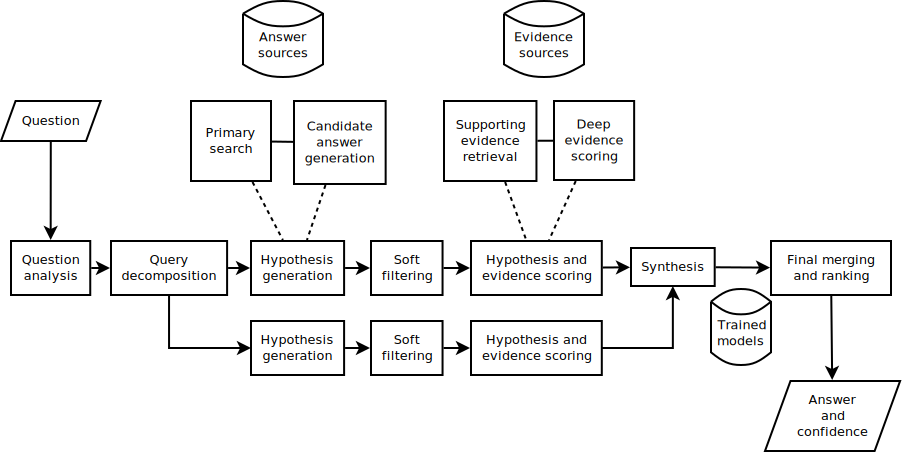
\includegraphics[width=12cm]{Pictures/DeepQA.pdf}
	\caption{Watson's high level architecture}
	\label{ch:rw:ml:watson}
\end{figure}



%----------------------------------------------------------------------------------------
%	DIALOGUE SYSTEMS
%----------------------------------------------------------------------------------------

\section{Dialogue Systems}

Research on dialogue systems has been carried on since the \textbf{early days} of Artificial Intelligence. A milestone in the early work on this field is ELIZA \citep{Weizenbaum:1966:ECP:365153.365168}, which provides the user with a basic human-like interaction based on pattern matching; Figure \ref{ch:rw:ds:ELIZA} shows an instance of these patterns.

Another example is the SHRDLU system \citep{winograd1971procedure}, which interfaces the user with a simple spatial domain by listening to the user's utterances (e.g.\ ``Would you please put the green pyramid in the box?"), and performing actions accordingly in the domain, resolving, if necessary, ambiguous or implicit references to the entities in it.

\begin{figure}
\begin{Verbatim}[frame=single]
["dream", 3, [
 ["*", [
     "What does that dream suggest to you ?",
     "Do you dream often ?",
     "What persons appear in your dreams ?",
     "Do you believe that dreams have something to do
      with your problem ?"
  ]]
]]
\end{Verbatim}
\caption{One of the patterns included in ELIZA's DOCTOR script. It simply tells the system that the user input can be answered with any of the given sentences, whenever it contains the word ``dream".}
\label{ch:rw:ds:ELIZA}
\end{figure}

\subsection{Task vs Nontaks}

According to \cite{Jokinen2009}, modern dialogue systems can be divided in \textbf{two main types}: task-oriented and nontask-oriented. Intuitively, systems in the first category are meant to deal with a specific task such as making a hotel booking, or booking a plane ticket; an example in this category is the MIT Mercury system, a vocal interface to a flight database \citep{Seneff:2000:DMM:1605285.1605288}. On the other hand, nontask-oriented systems are meant to engage in conversations without a specific purpose to fulfill, but the one of delivering a realistic simulation; ELIZA itself is an example of nontask-oriented dialogue system.

Task-oriented systems can be very simple, as simple and well-formalized the task is;  many applications, such as travel service or call routing, can be successfully solved by \textbf{slot-based} systems: each step of the conversation requires some pieces of information, modeled as slots, to be filled in by the user (departure city, arrival city, date, and so on); given the slots to be filled, the dialogue task can be solved with a formal grammar of interaction. As the complexity increases, more phenomena of human interaction have to be modeled, such as turn-taking, multimodality or grounding
%\ignore{CITE RAQUEL'S CHAPTER}
, as well as semantic structures such as quantification and negation; slot-based systems are not sufficient to model these scenarios \citep{Gabsdil03clarificationin}, that require more advanced frameworks such a the Information State Update (ISU) one, which will be tackled in \ref{ch:rw:ds:isu}.

\subsection{Information State Update Dialogue Management}\label{ch:rw:ds:isu}
The ISU approach to Dialogue Management, as it is described by \cite{TraumLarsson03p325}, can be seen as an attempt to reduce the gap between ``theories of dialogue that linguists or philosophers of language may devise and theories directly implemented in dialogue systems".

The linguistic and philosophical roots of this theory can be found in the notion of \textbf{common ground}, as it is defined by [STALNAKER CITE]; on Stalnaker's account, the common ground consists of an unstrucrured set of all the possible worlds that are compatible with the propositions asserted so far in the dialogue. A slightly more sophisticated formulation of the same concept comes from [LEWIS, CITE], who, drawing a parallel between dialogues and baseball, introduces the notion of ``conversational scoreboard", to keep track of the participants' moves. Even closer to the model of Traum and Larsson is \textbf{Ginzburg's dialogue gameboard} [CITATION]; one of the main differences between this model and the other two is represented by the inner structure of the scoreboard, which in Ginzburg is not just a set of propositions, but rather provides a structure made of facts, questions under discussion (QUD) and moves.

Traum and Larsson's notion of \textbf{Information State} takes Ginzburg's DGB one step further, by extending it with a formal representation of what Ginzburg calls the unpublished part of a dialogue partner's mental state (UNPUB-MS), and that will become the private part of the Information State. Figure \ref{ch:rw:ds:isu:ibisis} shows a simple Information State type, as it is implemented in the IBiS1 system \citep[p. 36]{Larsson02issue-baseddialogue}. It can be easily noticed that the IS is split in two sections, ``Private" and ``Shared", each of them containing formal representations of informational components: an agenda of actions being executed, a plan for future actions and a set of beliefs for the \textbf{private} part, the set of propositions in the common ground, a stack of questions under discussion, and the last utterance in the \textbf{shared} part.

The central concept of ISU-based systems is to \textbf{update} this, initially empty, Information State, according to the dialogue moves performed by the DPs. A \textbf{dialogue move} is tipycally a natural language utterance, but, in more complex systems, can also be a different form of interaction, like a gesture. The system detects this interactions, and is able to modify the IS accordingly (e.g.\ inserting a new question under discussion, or marking an action as completed, and so on) thanks to a set of \textbf{update rules}, and an \textbf{update strategy}, to decide on which rules to apply when more than one can be selected.

\begin{figure}
	\centering
	\includegraphics{Pictures/ibis1_is.png}
	\caption{Information State, as it is implemented in IBiS1}
	\label{ch:rw:ds:isu:ibisis}
\end{figure}

This work is relevant to us, as our software builds on the TDM dialogue management library (see \ref{ch:arch:TDM}), which implements the Information State Update framework.
% Chapter Template

\chapter{Architecture} % Main chapter title

\label{ch:arch} % Change X to a consecutive number; for referencing this chapter elsewhere, use \ref{ChapterX}

\lhead{Chapter \ref{ch:arch}. \emph{Architecture}} % Change X to a consecutive number; this is for the header on each page - perhaps a shortened title

%----------------------------------------------------------------------------------------
%	INTRO TEXT
%----------------------------------------------------------------------------------------

The outcome of this thesis project is \pname, a music player application that accepts English utterances as commands, adapts to utterances it has never been exposed to, and learns from them by possibly interacting with the user, thus expanding its initial knowledge of the language. The application has been written in Python 2.7, and consists of a client application for the existing OpenTDM dialogue management library. Such a library supports basic dialogue management based on the Information State Update approach, but has no support for grounding or flexible understanding of unknown sentences. Therefore, TDM has been extended with the Language Unit module, that introduces these capabilities.
% TODO: mention interpretation and generation models with ref to Staffan A.9

Section \ref{ch:arch:client} describes the \pname client, Section \ref{ch:arch:TDM} describes the OpenTDM library, and Section \ref{ch:arch:LU} describes the Language Unit module.


%----------------------------------------------------------------------------------------
%	CLIENT
%----------------------------------------------------------------------------------------

\section{The Client Application} \label{ch:arch:client}
\pname is a client application for OpenTDM, a dialogue management library based on the work by \cite{Larsson02issue-baseddialogue}. An OpenTDM application can be seen as a container for domain-specific \textbf{parameters} for the dialogue manager. These parameters consist of:
\begin{itemize}
\item A \textbf{device} class, containing variables and methods that directly control the actions of the application. The \textit{device} file of a music player application will contain, for instance, variables holding the current playlist, or the current volume level, and methods to play/stop the music, lookup for a song and so forth.
\item An \textbf{ontology}, whose main purpose is to define predicates and actions that will be used at dialogue management level. In the case of \pname, an example of predicate is \texttt{current\_song(X)}, that identifies the song currently being played (note that such a predicate must be mirrored in the device file as a variable\footnote{The actual implementation consists of an inner \texttt{current\_song} class of the device class, which access the proper, private, variable of the device file through a \texttt{perform()} method. The reasons that led to such an implementative choice were not made known by the authors of OpenTDM.}); an example of action is \texttt{increase\_volume} that, intuitively, identifies the action of increasing the volume (actions are mirrored as well in the device class, in the same way predicates are).
\item A \textbf{domain} file, whose main purpose is to contain the list of plans that will control the dialogue episodes. For instance, the TOP plan of an application is to find out what the user wants to do. Another example of a plan in \pname is the \texttt{increase\_volume} plan: step 1 of the plan is to ask the user for how much the volume should be increased, step 2 is to perform the actual action through the device.

Figure \ref{ch:arch:client:increaseplan} shows the plan item, as it is defined in the application domain: we notice that the \texttt{plan} section is a list of two elements, a \texttt{findout()} function, that will ask the user for the amount of volume to increase, and a \texttt{dev\_perform()} function, that will fire the volume increasing method in the device.
\begin{figure}
\begin{Verbatim}[frame=single]
{
  "goal": "increase_volume",
  "plan": [
              "findout(?X.volume_to_increase(X))",
              "dev_perform(
			   IncreaseVolume,
			   MplayDevice,
			   {postconfirm=True}
			  )"
	   ],
  "postconds": ["done(IncreaseVolume)"]
}
\end{Verbatim}
\caption{The \texttt{increase\_volume} plan of \pname.}
\label{ch:arch:client:increaseplan}
\end{figure}
\item A \textbf{grammar} implemented using the Grammatical Framework\footnote{http://www.grammaticalframework.org/} \citep{citeulike:346448}. This part will not be discussed, since, as it is explained in Section \ref{ch:arch:LU}, the Grammatical Framework in OpenTDM has been replaced with a specifically created module called Language Unit (LU). However, the purpose of the two modules is the same, and covers what in Section \ref{ch:introduction:arch} we called language understanding and response generation. That is, mapping natural language user utterances to their formal representations and vice versa.

In the example of Figure \ref{ch:arch:client:increaseplan}, a language understanding use of the Language Unit is to take, for instance, the input sentence ``Increase the volume" and turn it into a \texttt{request(increase\_volume)} user move, that will be used to load the proper plan from the domain. A response generation use of the LU will be, for instance, to take the \texttt{ask(?X.volume\_to\_increase(X))} system move (that will be produced by the \texttt{findout()} part of the plan), and turn into a sentence like ``By how much you want the volume to be increased?".
\end{itemize}

The dialogue management logic is left to OpenTDM, that will be discussed in the next section.


%----------------------------------------------------------------------------------------
%	TDM
%----------------------------------------------------------------------------------------

\section{OpenTDM} \label{ch:arch:TDM}
OpenTDM is a \textbf{dialogue management library} developed and maintained by Talkmatic\footnote{http://talkamatic.se/} based on the Information State Update framework (see \ref{ch:rw:ds:isu}). OpenTDM is a Python 2.7 port of the TRINDI Dialogue Move Engine Toolkit \citep{Larsson:2000:ISD:973935.973943}, that was originally implemented in Prolog.

The purpose of OpenTDM is to keep track of the Information State (IS), updating it on new user utterances, and planning the system moves accordingly. This is done by applying the standard ISU rules and policies \citep{Larsson02issue-baseddialogue} to the resources defined by the application (ontology, domain, device and language). Appendix \ref{a:isu} presents an example of how SVPlay's information state changes during an interaction with the user.

It is worth to note that OpenTDM is not yet available to the public, and comes with \textbf{no documentation}. This has significantly limited us in the design of the solution, preventing us from both implementing elaborated extensions of it (e.g.\ more complex learning interactions than the ones described in Chapter \ref{ch:interaction}), and respecting the software architecture best practicses, as many of the OpenTDM extensions that we have implemented rely consistently on hacks and temporary workarounds.

%----------------------------------------------------------------------------------------
%	LU
%----------------------------------------------------------------------------------------
\section{The Language Unit} \label{ch:arch:LU}
The Language Unit (LU) is a Python library that has been specifically created to support \pname's utterances understanding ability, serving as a drop-in replacement for the Grammatical Framework, that is used in the main OpenTDM branch. The purpose of this library is to perform the classification task as it has been defined so far, that is, assigning every input sentence to its correct meaning label.

\subsection{Language}
The \texttt{Language} class is the main class of LU, its purpose is to model a natural language under the following \textbf{abstraction}: a Language is defined by a finite set of Meanings (labels); a Meaning is defined by a finite set of Sentences expressing that Meaning. As an example, the \pname language consists of a number of meanings, each of them defining an action for the application to perform; one of these meanings can be the one to pause the current song; this meaning will be realized by a number of English sentences, like ``Pause the song", ``Suspend the music", or ``Pause the current track". For the purpose of language understanding, a Sentence can be brougth down to any of its (linguistic or non-linguistic) constituents called Chunks or Phrases. A chunk is formed by one or more Words.

The following are the main capabilities implemented in the Language class:
\begin{itemize}
	\item \textbf{Load} and \textbf{save} languages. Each OpenTDM application must define a \texttt{language/} folder where the language is stored, in the form of a \texttt{.l} file. Such a file is just a dump of all the meanings and their example sentences. Since the language  can evolve through learning, applications' language files are updated every time the application is run and dialogue interactions are performed. This update consists of adding new examples to meanings (unknown sentences from the user that have been understood with a good degree of confidence) and updating the usage count of the known examples that have been processed during the interaction with the user.
	\item \textbf{Learn} a sentence. When a new labeled example (a sentence with its meaning label) is provided, the knowledge of the language is extended. This is done adding the new sentence to the list of sentences realizing that meaning, and drawing statistics (e.g. the frequency of a certain word/phrase in the given meaning) to improve the model of the meaning. Note that, when a language is loaded for the first time, every sentence in it is run through the learning procedure to initialize the statistics.
	\item \textbf{Understand} an input sentence. The core task of the Language Unit is to associate an input sentence with its correct meaning. While this operation is trivial when the input sentence is already present in the language, it becomes hard for unknown examples. In this latter case the LU computes a score for the sentence against each of the meanings that are present in the language; the meaning that achieves the best score is given as an output, along with the score itself, representing the degree of confidence for the output to be correct. The way sentences are scored is presented in the next section.
\end{itemize}

\subsection{Scores} \label{ch:arch:LU:scores}
The way the Language Unit understands a sentence is based on a number of nested comparisons, resulting into as many comparison scores. A \textbf{score} is a linear combination of separate features. The top-level task is to score the sentence against every meaning in the application database; for each of them a \textbf{Meaning Score} (see \ref{ch:arch:LU:scores:meaning}) is computed, representing how likely the input sentence is to be a realization of that meaning. This score is based on the similarity of the input sentence with the known sentences realizing the meaning; the \textbf{Sentence Score} (see \ref{ch:arch:LU:scores:sentence}) represents the similarity between two sentences. This score is based on how similar the (linguistic or non-linguistic) components of the two sentences are; any sub-string of a sentence is called Chunk, and the \textbf{Chunk Score} (see \ref{ch:arch:LU:scores:chunk}) represents the similarity between two chunks. The Chunk Score is based on the similarity of the words contained in the two chunks; the \textbf{Word Score} (see \ref{ch:arch:LU:scores:word}) represents the similarity between two words.

\subsubsection{The \texttt{Score} Data Structure}
Scores in the application are modeled by the \textbf{\texttt{Score} class} (\texttt{lu/score/\_\_init\_\_.py}). A \texttt{Score} object defines the following \textbf{fields}:
\begin{itemize}
	\item \texttt{Score.features}, an array of N features that are used to form the final score. A feature is represented as a floating-point (\texttt{float}) number.
	\item \texttt{Score.weights}, an array of N weights that are used in the linear combination of features to form the final score. A weight is also represented as a floating-point (\texttt{float}) number. Weights are equally distributed by default, but they can be overridden with custom values. To this respect, an ideal scenario would be the one in which \textbf{optimal weights} for the features are determined with machine learning (\emph{meta-model learning}), as it will be described in Chapter \ref{ch:conclusions}. % TODO: REFINE CITATION, maybe also cite Watson
\end{itemize}
Implementation-wise, for the sake of efficiency, the Python \texttt{array} module\footnote{http://docs.python.org/2/library/array.html} is used instead of traditional lists and dictionaries. Such a module defines ``an object type which can compactly represent an array of basic values", directly based on their original C implementation. The acces to the elements of an \texttt{array} is positional. For this reason any instantiation of \texttt{Score} is recommended to define proper \textbf{constants} to access the single features.

The \texttt{Score} class also defines the following \textbf{methods}:
\begin{itemize}
	\item \texttt{Score.set\_feature(i, value)}, sets \texttt{value} as the value of the the $i$-th feature.
	\item \texttt{Score.get\_feature(i)}, returns the value of the the $i$-th feature.
	\item \texttt{Score.get\_score()}, returns the final score, as the weighted average of the features:
	\begin{displaymath}
		\sigma=\sum\limits_{i=1}^Nw_if_i
	\end{displaymath}
	Where $\sigma$ is the final score, $N$ is the total number of features, $f_i$ is the $i$-th feature and $w_i$ is the weight of the $i$-th feature.
\end{itemize}

Parallel to its class definition, any subclass of score must define a list $h = \{h_1, ..., h_N\}$ of procedures, called \textbf{hooks}, that compute the single features of the score, and a \textbf{factory} method, which runs the two elements to be compared through the feature hooks, fills a score object with the results and returns it. As an example, let's consider a fictional Word Score class, that scores the similarity of two English words, and that has only one feature, being the edit distance between the two words. In this case the hooks list will contain only one element ($h=\{h_1\}$), which is a pointer to a procedure \texttt{c\_edit\_distance(word\_from, word\_to)}, that returns the edit distance between two input words. The factory function \texttt{get\_score(word\_from, word\_to)}\footnote{Not to be confused with the \texttt{Score.get\_score() method.}} will instanciate an empty score object, and will assign the result of the computation of every feature hook $h_i$ to the corresponding feature $f_i$; therefore, the only feature of the score, representing the edit distance, will be filled with the result of \texttt{c\_edit\_distance}.

The following sections describe how the \texttt{Score} class is \textbf{extended} to model the different levels of scores that were introduced above.

\subsubsection{Meaning Score} \label{ch:arch:LU:scores:meaning}
A Meaning Score $\sigma_M(s,m)$ represents the likelihood of the sentence $s$ to be a realization of the meaning $m$. It is represented in the application by the \texttt{MeaningScore} class (\texttt{lu/score/meaning.py}), which is a subclass of \texttt{Score}. Such a class defines the following \textbf{three features}:
\begin{itemize}
	\item \texttt{MeaningScore.MAX\_SSCORE} - The best similarity score between the input sentence and one of the sentences that realize the meaning.
	\begin{displaymath}
		\sigma_{M,\text{MAX\_SCORE}}(s,m) = \max{\sigma_S(s,s_i)}
	\end{displaymath}
	Where $\sigma_{M,\text{MAX\_SCORE}}$ is the value of the feature, $s$ is the input sentence, $m$ is the meaning $s$ is scored against, $\sigma_S$ is a Sentence Score (see Section \ref{ch:arch:LU:scores:sentence}) and $s_i \in m$ is one of the know sentences that realize $m$.
	
	\item \texttt{MeaningScore.AVG\_SSCORE} - The average similarity score between the input sentence and the sentences that realize the meaning.
	 \begin{displaymath}
		\sigma_{M,\text{AVG\_SCORE}}(s,m) = \frac{\sum\limits_{i=1}^N{\sigma_S(s,s_i)}}{N}
	\end{displaymath}
	Where $N$ is the number of known sentences that realize $m$.
	
	\item \texttt{MeaningScore.ML\_CCSUM} - The sum of the class-conditional probabilities of every possible sub-string of $s$.
	 \begin{displaymath}
		\sigma_{M,\text{ML\_CCSUM}}(s,m) = \sum\limits_{c_s \in s}{p(c_s|m)}
	\end{displaymath}
	Where $c_s \in s$ is a sub-string (chunk) of $s$ and $p(c_s|m)$ is the class-conditional probability of $c_s$ respect to the meaning $m$, that is, the relative frequency of $c_s$ in the known sentences that realize $m$.
\end{itemize}

\subsubsection{Sentence Score} \label{ch:arch:LU:scores:sentence}
A Sentence Score $\sigma_S(s_\text{from},s_\text{to})$ represents how likely sentences $s_\text{from}$ and $s_\text{to}$ are to realize the same meaning.
% or maybe "how similar the meaning of s1 is to the one realized by s2", or maybe just "how similar s1 and s2 are"
Even though more features could be considered to measure this value, at the moment a Sentence Score is defined as the Chunk Score (see Section \ref{ch:arch:LU:scores:chunk}) $\sigma_C(c_1,c_2)$, where $c_1$ is the chunk spanning the whole $s_\text{from}$, and $c_2$ is the chunk spanning the whole $s_\text{to}$.

\subsubsection{Chunk Score} \label{ch:arch:LU:scores:chunk}
A Chunk Score $\sigma_C(c_\text{from},c_\text{to})$ represents how similar the chunk $c_\text{from}$ is to the chunk $c_\text{to}$. In the context of this thesis, a Chunk is defined as any possible substring of a sentence $s$ (not necessarily syntactic constituents), including $s$ itself. As an example, the sentence 

\enumsentence{``Execute order 66"} contains the chunks ``Execute", ``order", ``66", ``Execute order", ``order 66" and ``Execute order 66".

In the application, a Chunk Score is represented by the \texttt{ChunkScore} class (\texttt{lu/score/chunk.py}), which is a subclass of \texttt{Score}. Such a class defines the following \textbf{five features}:
\begin{itemize}
	\item \texttt{ChunkScore.AAVG} - The maximum, over all the possible 2-splits of the input chunks, of the arithmetic averages of the best alignment scores.
	\begin{displaymath}
		\sigma_{C,\text{AAVG}}(c,d) = \max\limits_{i,j}\left\{\frac{ \max\left\{\sigma_C(c_0^i,d_0^j), \sigma_C(c_0^i,d_{j+1}^M)\right\} + \max\left\{\sigma_C(c_{i+1}^N,d_0^j),\sigma_C(c_{i+1}^i,d_{j+1}^M)\right\}}{2}\right\}
	\end{displaymath}
	Where $c$ is a chunk of $N$ words, $d$ is a chunk of $M$ words, $c_a^b$ is a sub-string of $c$ spanning from the $a$-th word of $c$ to the $b$-th word of $c$, $i\in(0,N]$ and $j\in(0,M]$.
	
	By \textbf{2-split} of a chunk we mean a split of it in two sub-strings of arbitrary size; as an example, a 2-split of the chunk $c$ ``Increase the volume" can be \enumsentence{$|\text{ Increase } | \text{ the volume } |$} In this case we refer to ``Increase" as $c_1^1$ (the sub-string of $c$ spanning from position 1 to position 1), and to ``the volume" as $c_2^3$.
	
	Given two chunks that have been split in two parts each, each sub-string of one can be associated with a sub-string of the other\footnote{Since a sub-string can be a single word, as well as the whole chunk, we have two special cases to consider. Firstly, a word can be scored against another word; in this case the returned score is not a Chunk Score, but rather a Word Score (see \ref{ch:arch:LU:scores:word}). Then, it may happen that the whole first chunk is scored against the whole second chunk; this is prevented by the algorithm, as it would result in an infinite loop.}. For example, given the chunks $c$ ``increase the volume" and $d$ ``turn up the volume", an ideal behaviour would be to associate $c_1^1$ (``increase") with $d_1^2$ (``turn up") and $c_2^3$ (``the volume") with $d_3^4$ (``the volume"). Such an association is what we call an \textbf{alignment}\footnote{Note that, while ideally every $c_i^j$ could be aligned with 0, 1 or 2 $d_k^l$ and vice versa, due to implementation restrictions the software allows a $c_i^j$ to be aligned with only one $d_k^l$, where every $d_k^l$ can be aligned to 0, 1 or 2 $c_i^j$. }, and it produces two Chunk Scores (in the case of the example, $\sigma_C(c_1^1,d_1^2)$ and $\sigma_C(c_2^3,d_3^4)$).
	
	Thus, for every possible combination of 2-splits of the two input sentences, a number of alignments is possible, each of them associated with two Chunk Scores. For each combination of 2-splits the alignment that produces the best scores is selected; once this has been determined, the external maximization is performed, so that the best combination of 2-splits is returned.
	
	It is worth to note that the value of this feature \textbf{builds recursively} on the scores of these smaller chunks, chosing the split and the alignment for the final score to be maximized. For this purpose a special algorithm called M2 has been defined, a more detailed description of it can be found in Chapter \ref{ch:M2}.
	
	\item \texttt{ChunkScore.LEN} - Sets a preference for big chunks over short ones.
	\begin{displaymath}
		\sigma_{C,\text{LEN}}(c,d) = 1-\frac{1}{\min(|c|,|d|)+\alpha}
	\end{displaymath}
	Where $|c|$ is the length in words of $c$, $|d|$ is the length in words of $d$, and $\alpha$ is a smoothing constant.
	
	\item \texttt{ChunkScore.STRAIGHT} - Sets a preference for straight alignments over crossed ones.
	\begin{displaymath}
		\sigma_{C,\text{STRAIGHT}}(c,d) = \begin{cases} 1, & \mbox{if } n\mbox{ streight alignment} \\
		                                                0.5, & \mbox{if } n\mbox{ half-straight alignment} \\
		                                                0, & \mbox{if } n\mbox{ crossed alignment} \end{cases}
	\end{displaymath}
	Where, under the assumption that the best alignment has been determined by \texttt{ChunkScore.AAVG}, a \textbf{straight} alignment happens when the first sub-string of $c$ is aligned to the first sub-string of $d$, and the second sub-string of $c$ is aligned with the second sub-string of $d$; a \textbf{half-straight} alignment happens when both the sub-strings of $c$ are aligned to the same sub-string of $d$; a \textbf{crossed} alignment happens when the first sub-string of $c$ is aligned to the second sub-string of $d$, and the second sub-string of $c$ is aligned with the first sub-string of $d$.

	\item \texttt{ChunkScore.ML\_CFREQ} - The Chunk Likelihood. This features is meant to enforce good linguistic splitting of the input chunks, as it sets a preference for chunks that occur more in the language base (eg. the chunk ``the volume" is supposed to occur more often that ``increase the"). Such a value is based on Machine Learning from previous examples, and it is implemented as the sum of the relative counts of the two chunks. A more detailed explanation of this will be given in \ref{ch3:ml:cl}.
	
	Note that this feature does not measure the goodness of the alignment, but should rather be considered as a \textbf{language modeling} feature; this has the drawback of contributing to the overall score every times the two input chunks are linguistically plausible, even if they should not be aligned together. Furthermore, a good amount of training data is required to prevent \textbf{data sparsity} problems. Both of these issues will be addressed in \ref{ch3:ml:cl} as well.

	\item \texttt{ChunkScore.ML\_AFREQ} - The Alignment Likelihood. Such a value is based on Machine Learning from previous examples, and it is implemented as the relative count of the times the two input chunks have been found aligned together. A more detailed explanation of this feature will be given in  \ref{ch3:ml:al}. 
\end{itemize}

\subsubsection{Word Score} \label{ch:arch:LU:scores:word}
A Word Score $\sigma_W(w_\text{from},w_\text{to})$ represents how similar the word $w_\text{from}$ is to the word $w_\text{to}$. It is represented in the application by the \texttt{WordScore} class (\texttt{lu/score/word.py}), which is a subclass of \texttt{Score}. Such a class defines the following \textbf{five features}:
\begin{itemize}
	\item \texttt{WordScore.EQUALS} - Boolean equality.
	\begin{displaymath}
		\sigma_{W,\text{EQUALS}}(w_\text{from},w_\text{to}) = \begin{cases} 1, & \mbox{if } w_\text{from} = w_\text{to} \\
		                                                                    0, & \mbox{otherwise} \end{cases}
	\end{displaymath}
	
	\item \texttt{WordScore.EDIT\_DISTANCE} - The edit distance is a measure of string-wise similarity defined by \cite{levelshtein-66-binary}: the more two strings are similar, the less their distance.
	\begin{displaymath}
		\sigma_{W,\text{EDIT\_DISTANCE}}(w_\text{from},w_\text{to}) = 1-f(w_\text{from},w_\text{to})
	\end{displaymath}
	Where $f(w_\text{from},w_\text{to})$ is the edit distance between $w_\text{from}$ and $w_\text{to}$, as it is implemented in the Python Natural Language ToolKit \citep{Loper:2002:NNL:1118108.1118117}.
	
	\item \texttt{WordScore.POSITION\_DISTANCE} - inversely proportional to the difference between the position of $w_\text{from}$ in its sentence and the position of $w_\text{to}$ in its sentence.
	\begin{displaymath}
		\sigma_{W,\text{POSITION\_DISTANCE}}(w_\text{from},w_\text{to}) = \left(\frac{1}{|p(w_\text{from})-p(w_\text{to})|}\right)^\alpha
	\end{displaymath}
	Where $p(w)$ is the position of the word $w$ in its sentence, and $\alpha$ is a free parameter.
	
	\item \texttt{WordScore.WN\_MAX\_PATH\_SIMILARITY} - The length of the shortest path between the two words in the WordNet onthology \citep{Miller:1995:WLD:219717.219748}. This measure is implemented in the NLTK as well.
	
	\item \texttt{WordScore.ML\_AFREQ} - The Alignment Likelihood. This feature has already been described in \ref{ch:arch:LU:scores:chunk}.
\end{itemize}

\section{Summary}\label{ch:arch:LU:summary}
In this chapter we described the architecture of \pname in general, and of its sentence scoring system in particular.

\pname is a client application for the \textbf{OpenTDM} library. The application defines its plans, language and device actions, while OpenTDM takes care of the dialogue management, being the execution of the plans that are appropriate to the context (e.g.\ to increase the volume when the user issues ``Increase the volume").

The \textbf{Language Unit} is a drop-in replacement for OpenTDM's default language processing system (the Grammatical Framework); its main duty is to provide flexible understanding of user utterances. This is done through nested, score-centric, feature-based comparisons between the input sentence and the sentences representing each of the meanings available in the application. The interpretation of an input sentence is given as a list of Meaning Scores, representing how likely the sentence is to realize each of the meanings.

Figure \ref{scoresbreakdown} shows a breakdown of a \textbf{Meaning Score}. From this figure we can see that a Meaning Score is made of three features, one of which relies on Machine Learning data (\texttt{ML\_CCSUM}), and the other two (\texttt{MAX\_SSCORE} and \texttt{AVG\_SSCORE}) are based on single Sentence Scores, representing the similarity between the input sentence and the ones in the meaning. A \textbf{Sentence Score} is just a Chunk Score. A \textbf{Chunk Score} represents the similarity between two chunks of text, and has five features; two of them make use of ML data (\texttt{ML\_CFREQ} and \texttt{ML\_AFREQ}), and one is derived either from other, smaller, Chunk Scores, or from a Word Score (the way smaller scores are combined into a bigger one will be better explained in the next chapter). A \textbf{Word Score} has four features, one of which (\texttt{ML\_AFREQ}) makes use of ML data.

The result of every comparison is also used to update the ML model (e.g.\ incrementing the count of the chunks that have been encountered). This aspect will be tackled in \ref{learning}.


\begin{sidewaysfigure}
\includegraphics[width=23cm]{Pictures/scores_diagram.pdf}
\caption{Scores' structure}
\label{scoresbreakdown}
\end{sidewaysfigure} 

\chapter{Sentence similarity computation} % Main chapter title

\label{ch:M2} % Change X to a consecutive number; for referencing this chapter elsewhere, use \ref{ChapterX}

\lhead{Chapter \ref{ch:M2}. \emph{The M2 matching algorithm}} % Change X to a consecutive number; this is for the header on each page - perhaps a shortened title

In the context of sentences \textbf{classification}, where the task is to label an unknown input sentence with the correct meaning, and each meaning is defined by a set of representative natural language sentences (as it was defined in the Introduction), one crucial point is to measure the similarity of the input sentence with each of the sentences defining each meaning.

Computing a \textbf{similarity score} between two natural language \textbf{sentences} is not a trivial problem. Many features can be taken into account to solve it, such as the syntactic structure of the sentence, or the meaning of the single words, or their order; all of these features are informative respect to the meaning of the sentence, and it is reasonable to assume they are all considered by humans solving the same task. Here we describe a recursive, dynamic programming \textbf{algorithm} for sentence comparison aimed to exploit word-based information, as well as the syntactic one, expressed in the form of unsupervised learned binary trees.

% A bit more on literature, relation to the work would be nice..

The algorithm presented in this thesis aims to provide a similarity measure for two sentences $s_1$ and $s_2$ featuring many of the ideas that have proven to be successful in recent developments of Computational Linguistics. The following are some of the key insights of the algorithm:

\begin{itemize}
\item \textbf{Every possible} sub-sentence of $s_1$ is compared with every possible sub-sentence of $s_2$.
\item A score between two chunks of text is build \textbf{recursively} on the best matches of smaller chunks, and always brought down to scores between single words.
\item \textbf{Dynamic programming} is used to increase the efficiency of the algorithm, preventing it from computing the same result two times.
\item Other than the similarity score, the algorithm outputs the most probable chunking of each sentence in the form of an unlabeled binary \textbf{parse tree}.
\item Other than the similarity score and the parse trees, the algorithm outputs the most likely \textbf{alignment} between the chunks of the two sentences.
\item Every score is expressed as a linear combination of \textbf{features}, designed to be independent and extensible.
\item The partial computations of the algorithm can be stored and further used to implement a learning model.
\end{itemize}

%Document structure
This chapter is \textbf{structured} as follows. Section \ref{algo} describes the algorithm theoretically. %and in a better world a complexity analysis
%Section \ref{example} walks through a toy example.
Section \ref{learning} describes possible extensions and improvements. Section \ref{conclusions} draws the conclusion of the paper.

\section{The M2 matching algorithm} \label{algo}
\begin{algorithm}
  \SetKwData{Left}{left}
  \SetKwData{Up}{up}
  \SetKwFunction{WWScore}{$\tau$}
  \SetKwFunction{CCScore}{$\tilde{\sigma}$}
  \SetKwFunction{Length}{Length}
  \SetKwFunction{Split}{Split}
  \SetKwFunction{Set}{Set}
  \SetKwFunction{Append}{Append}
  \SetKwFunction{Max}{Max}
  \SetKwInOut{Input}{input}
  \SetKwInOut{Output}{output}
  \SetKw{In}{in}

\Indm  
  \Input{$c_1,c_2$ chunks of text; $T$ partial results table}
  \Output{$\sigma(c_1,c_2)$ Similarity score between $c_1$ e $c_2$}
\Indp
  \BlankLine
  \uIf{c1,c2 are words}{ \label{main:bc1}
	  \Return{\WWScore{$c_1,c_2$} \label{main:bc2} }
  }
  \BlankLine
  $S\leftarrow[\ ]$\; \label{main:cinit}
  \For{$i\leftarrow 1$ \KwTo \Length{$c_1$}}{ \label{main:loopi}
    $C_1 \leftarrow $ \Split{$c_1$,i}\; \label{main:spliti}
		\For{$j\leftarrow 1$ \KwTo \Length{$c_2$}}{ \label{main:loopj}
		\lIf{i=\Length{$c_1$} and j=\Length{$c_2$}}{break} \label{main:break}
		\BlankLine
		$C_2 \leftarrow $ \Split{$c_2$,j}\; \label{main:splitj}
		\BlankLine
		\ForEach{$sc_1$ \In $C_1$}{ \label{main:fe1}
			\ForEach{$sc_2$ \In $C_2$}{ \label{main:fe2}
				\uIf{$T[sc_1,sc_2]=\emptyset$}{$T[sc_1,sc_2] \leftarrow \sigma(sc_1,sc_2,T)$ \label{main:tabass} \label{main:tupdate}}
			}
		}
		\BlankLine
		\Append{$S$,\CCScore{$C_1,C_2,T$}} \label{main:cappend}
 }
	}
	\BlankLine
	\Return \Max{$R$} \label{main:return}
\caption{The main algorithm\label{main}}
\end{algorithm}

Algorithm \ref{main} contains the main loop of the sentence scoring algorithm. Before entering the details of it, it is necessary to say that:
\begin{itemize}
\item The input $c_1,c_2$ can be any \textbf{chunks} of text because, while the algorithm is called with two sentences in input, it will recursively call itself on every possible chunk extracted from the two sentences.
\item The input $T$ (T for Table) is a data structure holding the intermediate results of the algorithm. As we can infer from line \ref{main:tabass} of Algorithm \ref{main}, $T[c_1,c_2]=\sigma(c_1,c_2)$
\item $\tau(c_1,c_2)$ returns a similarity score between two words. This score is a linear combination of independent features. At the moment, the following features are taken into account:
\begin{itemize}
\item Equality (boolean) -- 1 if $c_1=c_2$, 0 otherwise
\item Edit distance -- $1-d$, where $d$ is the Levelshtein distance \citep{levelshtein-66-binary} between $c_1$ and $c_2$, as it is implemented in NLTK \citep{Loper:2002:NNL:1118108.1118117}
\item Difference in position -- $(1/|p_{c_1}-p_{c_2}|)^\alpha$, where $p_{c_i}$ is the position of $c_i$ in the sentence, and $\alpha$ is a free parameter.
\item Wordnet \citep{Miller:1995:WLD:219717.219748} Path Length similarity, as it is implemented in NLTK
\end{itemize}
The weights of the single features, now static, are meant to be trained through Machine Learning
\item \texttt{Length($c$)} returns the number of words contained in the chunk $c$
\item \texttt{Split($c,i$)} returns a list of two chunks, one containing the words of $c$ from the first to the $i$th, and the other containing the words of $c$ form the $(i+1)$th to the last.

If the $i$th word is the last word of $c$, it returns a list containing the only element $c$.
\item \texttt{Append($L,x$)} is the standard \emph{append} operation for lists, adding the element $x$ in the last position of the list $L$.
\item $\hat{\sigma}(C_1,C_2,T)$ returns the score of $c_1,c_2$ \textbf{given} a particular 2-split of the two chunks. Such a score is computed combining the ones of the smaller constituents of $c_1,c_2$, which are required to be already present in the table T.

The score is again the linear combination of independent features, leaving its implementation open and extensible.

At the moment the only feature being employed is the average of the scores of the best alignments of the sub-chunks in $C_1$ with the ones in $C_2$.

For example, given $C_1=[\text{"increase","the volume"}]$ and $C_2=[\text{"raise"},\\ \text{"the volume"}]$, "increase" is likely to achieve the best score with "raise" (eg. $T[\text{"increase","raise"}]=0.8$), as well as "the volume" will be aligned with "the volume" ($T[\text{"the volume","the volume"}]=1$)). The score of "increase the volume" and "raise the volume", in this particular splitting, will thus be the average of the two, 0.9.
\end{itemize}
After these premises it is relatively easy to walk through the pseudo-code of Algorithm \ref{main}. Lines \ref{main:bc1} and \ref{main:bc2} handle the base case, that is, when the algorithm is run on \textbf{two words}; in this case the result of the Word Similarity function, which is described above, is returned.

At line \ref{main:cinit} the list of \textbf{candidate results} is initialized as an empty list. This is because more than one score will be computed for $c_1$ and $c_2$, the maximum of which will be returned as a result.

Lines \ref{main:loopi} and \ref{main:loopj} define a nested loop structure, which purpose is to update the two indexes $i$ (from the first to the last word of $c_1$) and $j$ (from the first to the last word of $c_2$) to cover \textbf{every possible combination} of word positions in the two input strings. These indexes are used to \textbf{split} the input chunks in smaller parts (lines \ref{main:spliti} and \ref{main:splitj}). As an example, if the input is given by $c_1=$"increase the volume", $c_2=$"raise the volume", the outer loop will produce the three possible values of $C_1$: ["increase","the volume"], ["increase the","volume"] and ["increase the volume"]; each of these values will be combined, in the inner loop, with the three possible values of $C_2$: ["raise","the volume"], ["raise the","volume"] and ["raise the volume"].

Note that, while it is reasonable to consider the entire $c_1$ and $c_2$ in the comparisons (eg. if $c_1=$"quit",$c_2=$"quit please", we'd want the whole $c_1$ to be associated with the "quit" sub-part of $c_2$), it is necessary to prevent the two entire $c_1$ and $c_2$ to be associated at the same time, thus producing an \textbf{infinite loop}; this is done in line \ref{main:break}.

The next part of the inner loop, from line \ref{main:fe1} to line \ref{main:fe2} combines every sub-chunk of $c_1$ ($sc_1 \in C_1$) with every sub-chunk of $c_2$ ($sc_2 \in C_2$); note that $C_1$ and $C_2$ contain either one or two elements. Every combination that is not present in the table is scored with a \textbf{recursive} call to the algorithm itself, and the resulting score is saved in the table (line \ref{main:tupdate}).

The last operation done in the loop, at line \ref{main:cappend}, is to combine the sub-scores that have just been scored in the table to compute the final score of this particular subdivision of $c_1$ and $c_2$. This is a \textbf{candidate score} for $c_1$ and $c_2$, and thus is appended to the list of candidate scores. As we already said, the definition of this combination is open; however it is most reasonable for the $\hat{\sigma}$ function to find the \textbf{best alignment} between the input sub-chunks, and provide a score based on it. It is clear that the definition of $\hat{\sigma}$ is crucial for getting sensible results from the algorithm. Furthermore, $\hat{\sigma}$ is the point where the algorithm can be extended with Machine Learning capabilities, that will be discussed in Section \ref{learning}.

At line \ref{main:return} the function returns the \textbf{maximum of the candidate} score, that is, the split that produced the best score (eg. for "increase the volume" vs "raise the volume", the score of "increase $\vert$ the volume" vs "raise $\vert$ the volume" is likely to produce a better score than "increase $\vert$ the volume" vs. "raise the $\vert$ volume"). Note that this decision determines the branching of one level of the recursion tree; once the algorithm is done computing the score between two sentences, a traceback of the selected splits can be interpreted as a parse tree for the two input sentences.

%\section{An example} \label{example}

\section{Machine Learning Possibilities} \label{learning}
The basic algorithm described in section \ref{algo} only deals with \textbf{static features} to measure similarities: the score of two words is derived from equality, edit distance, Wordnet path length and so on; the score of chunks is the average of the scores of the best alignments of their components.

In this section I address the question whether it is possible, and how, for the algorithm to \textbf{learn} from the sentences it is parsing. In other words, given a sentence of which I know the meaning, how can I use this information to improve the way I process new sentences?

Here I consider \textbf{three features} based on Statistical Language Processing methods to address this problem: chunk likelihood, class-conditional chunk weight and alignments likelihood.

\subsection{Chunk likelihood} \label{ch3:ml:cl}
% Relative frequency across all sentences
% Used to select good chunks
Let's consider the following pair of sentences:
\begin{quote}
Pump up the volume\\
Turn up the volume
\end{quote}

As an English-speaking human being I immediately associate the phrase "pump up" with "turn up" and "the volume" with its analogue. One of the reasons I make this association rather than, for instance, associating "pump" with "turn" and "up the volume" with its analogue, is that I have good experience of the phrase "the volume" being used in different contexts, while fewer times I encounter "up the volume".

Thus a feature that can be useful to \textbf{enforce good chunking} of the input sentences is the likelihood of a chunk of text (where a chunk is defined as either a word or a combination of chunks). This feature can be modeled as the relative count of each chunk in the whole pool of the ones that have been recorded:
$$
l(c)=\frac{\text{\# of }c}{\text{\# of total chunks}}
$$

Note that this feature is completely unsupervised, in that it does not require a Meaning label to be computed.
\subsection{Class-conditional chunk weight} \label{ch3:ml:cc}
% frequency in class / frequency overall
% Used to weight more chunks that are representative for one class
Let's consider the following three sentences:
\begin{quote}
Increase the volume\\
I would appreciate if you could increase a bit the the volume\\
Decrease the volume
\end{quote}

With a reasonable approximation, the first two sentences have the same meaning, while the last says the opposite, although the first and the last sentence are much more similar from a syntactic point of view. Nevertheless, no English speaker would bother wondering about hidden meanings behind phrases like "I would appreciate", or "if you could": everyone could tell that the second sentence is no more than the first one, with some more formal dressing.

Especially, when I listen to the second sentence, I can immediately locate "increase" and "the volume" as the most informative phrases, while filtering out the rest as less relevant. One of the reasons I am able to do this is that I have memory of "I would appreciate if you could" used in sentences conveying lots of different meanings, while "increase" is likely to appear only in situations where something is increased.

A feature that could be useful to spot the \textbf{informativeness} of chunks can be the conditional probability of the chunk, given a certain meaning:
$$
l(c|m)=\frac{\text{\# of }c\text{ in }m}{\text{\# of }c}
$$

This feature can be used to weight the score of different chunks in the sentence, so for more informative chunks to influence more of the total score mass.
%l(c|m,M)?
\subsection{Alignment likelihood}\label{ch3:ml:al}
% Recursive score of alignments
% Used to align chunks correctly
Let's consider the following pair of sentences:
\begin{quote}
Skip this track \\
Jump over this song
\end{quote}
Again, English speakers can easily associate the meaning of "skip" with the one of "jump over", and the meaning of "track" with the one of "song".

One device that the algorithm uses to solve this problem is the \textbf{Wordnet} Path Lenght measure for word comparison. However, it has been noticed that this measure has its limits. In particular
\begin{itemize}
\item Not all the words are included in Wordnet
\item Being a static measure, it cannot be adapted to the domain
\item It has difficulties spotting antonyms
\end{itemize}
The alignment likelihood measure can be used to \textbf{enforce correct alignments} of different chunks.
$$
l(c_2|c_1)=\frac{\text{\# of }c_1-c_2\text{ alignments }}{\text{\# of }c_1\text{ alignments}}
$$
Note that, since no alignment labels are provided in the dataset (each sentence is labeled with a meaning, but its syntactic structure is hidden), this measure have to be trained in an unsupervised fashion. This problem shares a lot with the alignment likelihood in \textbf{Machine Translation}, even though here we can take advantage of the chunks sharing the same language (thus allowing some clever initialization of unsupervised methods with sensible guesses based, for instance, on Wordnet). On the other side our problem presents less precise training data, in that, while MT alignments are trained on sentence pairs, here we have a group of sentences sharing a same meaning; it can be argued that this cannot allow for strong syntactic assumptions.
% MT: T: more similar syntactic structure (label sentence by sentence)

\section{Summary} \label{conclusions}
In this chapter we described an algorithm to compare the similarity of two input sentences. Its main \textbf{advantages} are the concurrent consideration of many features like word meanings, position and overlapping, as well as the structure of the sentences, having the result in the form of aligned binary trees. The algorithm is recursive and exhaustive in that considers all the possible alignments of all the possible combinations of all the possible binary trees of the two input sentences, maximizing the efficiency with dynamic programming. Due to its modular structure, the algorithm can be easily extended with new features, allowing its integration with well-known Machine Learning techniques in Computational Linguistics (eg. Expectation-Maximization for computing word/phrase alignment probabilities).

There are some assumptions and \textbf{weak points} as well. First of all, the algorithm is inherently binary, in that every recursion step is made of a 2-split of the two input strings; this may have an effect in the way partial scores are combined. More generally, this "two times binary" recursive structure makes the features design task hard, since the effect of one operation is not easy to control over a potentially unlimited number of recursion steps. Also the number of parameters can become high, since each score is a linear combination of single features, requiring a separate Machine Learning training.

Lastly, this paper only describes the \textbf{backbone} of the algorithm, which is not yet ready for more formal tests on existing corpora. The main steps ahead before expecting good results from it include a better tuning and possible extension of the existing features  and the implementation of Machine Learning techniques to include alignment probabilities and more advanced statistical features for the chunks being compared (eg. their degree of informativeness).

%\begin{thebibliography}{9}

%\bibitem{achananuparp08}
%Palakorn Achananuparp, Xiaohua Hu, Xiajiong Shen. The Evaluation of Sentence Similarity Measures. Lecture Notes in Computer Science Volume 5182, 2008, pp 305-316

%\bibitem{udop}
%Rens Bod. Unsupervised parsing with U-DOP. CoNLL-X '06 Proceedings of the Tenth Conference on Computational Natural Language Learning, 2006, pp 85-92. 

%\bibitem{ibmmt}
%P. Brown, S. Della Pietra, V. Della Pietra, and R. Mercer (1993). The mathematics of statistical machine translation: parameter estimation. Computational Linguistics, 19(2), 263-311.

%\end{thebibliography}

% Chapter Template

\chapter{Interaction} % Main chapter title

\label{ch:interaction} % Change X to a consecutive number; for referencing this chapter elsewhere, use \ref{ChapterX}

\lhead{Chapter \ref{ch:interaction}. \emph{Interaction}} % Change X to a consecutive number; this is for the header on each page - perhaps a shortened title

%----------------------------------------------------------------------------------------
%	INTRO TEXT
%----------------------------------------------------------------------------------------
In the previous chapter we have seen how the Language Unit is able to associate utterances from the user with their most likely meaning; due to the nature of the problem, it cannot be guaranteed that the output meaning is actually the one intended by the user. However, we have also seen that such an association is the result of a fuzzy matching process, where the utterance receives a comparison score with each of the candidate meanings. When these scores are accurate, they provide an important \textbf{estimate of the confidence} whether the understanding is correct or not.

This chapter describes how the Language Unit exploits the information derived from the matching scores, to decide on whether a grounding interaction with the user is needed, and in case asking \textbf{pertinent questions} about the meaning of single sentence components. Also, an explanation of the \textbf{learning} process is given, that is, how the LU makes use of the user answers to update its knowledge about the language.

Section \ref{ch:interaction:mmw} describes how the best interaction policy is selected; Section \ref{ch:interaction:afl} explains how the software locates the minimal unclear constituents in the input sentence; Section \ref{ch:interaction:episode} deals with how the Language Unit interact with TDM to produce the grounding subdialogues; Section \ref{ch:interaction:learn} describes how the user answers are used to learn new information about the language.

%----------------------------------------------------------------------------------------
%	MEANING MATCHING WORKFLOW
%----------------------------------------------------------------------------------------

\section{Meaning Matching Workflow} \label{ch:interaction:mmw}
The first problem the Language Unit has to face, is to determine whether the understanding of an input utterance is good enough to be taken as correct, or it rather needs to be grounded with the user.

\subsection{Overview}
Let's consider the following situation:

\texttt{S> How can I help you? \\
U> what is the title of this song}

At this point, four different scenarios are possible:
\begin{enumerate}
	\item There is one best matching meaning, and its confidence score is high.
	\item There is one best matching meaning, but its confidence score is low.
	\item There are two or more meanings with a high confidence score.
	\item No meaning has a good confidence score.
\end{enumerate}
These different situations can be easily associated with as many \textbf{interaction policies}:
\begin{enumerate}
	\item Accept the best meaning without interaction.
	\item Ask whether the understanding of the best meaning is correct.
	\item Ask the user to disambiguate between the top candidates.
	\item Ask the user to rephrase his utterance.
\end{enumerate}

\subsection{Implementation: the \texttt{get\_plan()} Function} \label{ch:interaction:mmw:getplan}
The work of \textbf{deciding on the policy} to adopt is done by the \texttt{lu.learn.interaction} module, and especially by the \texttt{get\_plan()} function. This function takes a list of candidate meanings (and their confidence scores) as input, and outputs the plan that the dialogue manager should follow. In the case of TDM, the \texttt{get\_plan\_tdm()} function can be called, which returns the plan in the form of TDM-compatible dialogue moves\footnote{Due to the lack of documentation of the TDM code, it was not possible to integrate the grounding moves into the dialogue management library. Instead, a generic entry-point-move is used to start grounding subdialogues that are in fact controlled by the Language Unit. More details will be given in \ref{ch:interaction:episode}.}.

At first, \texttt{get\_plan()} \textbf{normalizes} the input scores, so that they sum up to 1. This allows us to compare them scores more easily\footnote{Note that, even if this is not done in the current implementation, one could think of using the un-normalized values to have an idea of the absolute confidence of the matches.}.

When the scores are normalized, \textbf{confidence thresholds} can be set in order to detect the four cases showed in \ref{ch:interaction:mmw}:
\begin{enumerate}
	\item The best score is greater than a constant $\alpha$. The value of $\alpha$ should be chosen so that $\alpha > 0.5$; in this way it is guaranteed that at most one meaning will be selected with maximum confidence.
	\item There is one and only one meaning whose confidence score is greater than a constant $\beta$, and yet smaller than $\alpha$. The value of $\beta$ should be chosen so that $\beta < \alpha$.
	\item There are two or more meanings whose confidence score is greater than $\beta$ and smaller than $\alpha$. In order to allow for this possibility, $\beta$ should be chosen so that $\beta < 0.5$
	\item None of the confidence scores is greater than $\beta$.
\end{enumerate}

In the experiments, the $\alpha$ and $\beta$ \textbf{constants} have been manually set to, respectively, 0.7 and 0.3. As it will be better discussed in Chapter \ref{ch:conclusions}, a better way to select these parameters would be to employ a meta-learning procedure to train the hypermodel for optimal performance.

At this point, \textbf{cases 1 and 4} are trivial to handle: \texttt{get\_plan()} will return the best matched meaning in the first case, and the meta-goal \texttt{\_rephrase}\footnote{Note that, since \texttt{get\_plan()} is called by TDM to interpret user utterances, formally this means ``User asked System to ask User to rephrase". A more elegant way of solving this issue would be to integrate rephrase requests in TDM, but this, again, was not possible due to lack of documentation.} in the latter. \texttt{\_rephrase} has the effect of terminating the interaction with the system utterance
\enumsentence{I do not quite understand what you mean, can you rephrase please?}

The following dialogue shows \pname dealing with the two situations that have just been described:

\texttt{S> How can I help you? \\
U> what is the current song \\
S> Running too fast, by Rehearsal Summer \\
S> How can I help you? \\
U> I like biscuits! \\
S> I do not quite understand what you mean, can you rephrase please?}

Cases \textbf{2 and 3} require a more sophisticated handling. In this cases, the Language Unit will first try to locate specific parts of the utterance that are particularly unclear (see \ref{ch:interaction:afl}), and then use them to produce a targeted clarification request to ground the correct meaning of the user utterance (see \ref{ch:interaction:episode}).

%----------------------------------------------------------------------------------------
%	MINIMAL AMBIGUOUS FRAGMENT
%----------------------------------------------------------------------------------------

\section{Ambiguous Fragment Location} \label{ch:interaction:afl}
When the Language Unit is not sure about the meaning of the user utterance, a procedure is used to reduce the uncertainty to the \textbf{smallest possible constituents} of the sentence. This is done by analyzing the similarity between the user utterance and the best matching sentence within each of the candidate meanings.

\subsection{Overview}
Let's consider, as an example, the meaning \texttt{ask(?X.current\_song(X))}, defined by the sentences in \ref{ch:interaction:afl:meaning}, and the question in \ref{ch:interaction:afl:whatisthis}. If this question matches this meaning, achieving its best score with the sentence in  \ref{ch:interaction:afl:meaningmatch}, the software should then return ``the current" from \ref{ch:interaction:afl:whatisthis} and ``this" from \ref{ch:interaction:afl:meaningmatch} as the minimal uncertain alignment, because all the other parts are \textbf{perfectly matched}. The way this especially unclear constituents are detected will de described in \ref{ch:interaction:afl:impl}.
\eenumsentence{\item What is the current song \label{ch:interaction:afl:meaningmatch}
			     \item Which song is playing
			     \item Which track is playing} \label{ch:interaction:afl:meaning}
\vspace{-0.5cm} %HACK
\enumsentence{What is this song? \label{ch:interaction:afl:whatisthis}} 
Of course, the algorithm should have a \textbf{margin of tolerance} as to the constituents whose match should be considered accepted. As an example, the sentence in \ref{ch:interaction:afl:whats} shouldn't raise concerns about the ``What's"/``What is" alignment, when compared against \ref{ch:interaction:afl:meaningmatch}; this is because, even though the match between ``What's" and ``What is" is not perfect, it is expected to achieve a sufficiently high score to be considered matched without questions.
\enumsentence{What's this song? \label{ch:interaction:afl:whats}}


\subsection{Implementation: the \texttt{locate\_fragments()} Function} \label{ch:interaction:afl:impl}
Algorithm \ref{ch:interaction:afl:algo} defines the \texttt{locate\_fragments()} function, which is used to locate, in the utterance from the user, the \textbf{constituents} that are especially unclear.

\begin{algorithm}
  \SetKwData{Left}{left}
  \SetKwData{Up}{up}
  \SetKwFunction{WWScore}{$\tau$}
  \SetKwFunction{CCScore}{$\tilde{\sigma}$}
  \SetKwFunction{from}{from}
  \SetKwFunction{to}{to}
  \SetKwFunction{getalignment}{get\_alignment}
  \SetKwFunction{getscore}{get\_score}
  \SetKwFunction{min}{min}
  \SetKwFunction{Length}{Length}
  \SetKwFunction{Split}{Split}
  \SetKwFunction{Set}{Set}
  \SetKwFunction{Append}{Append}
  \SetKwFunction{Max}{Max}
  \SetKwInOut{Input}{input}
  \SetKwInOut{Output}{output}
  \SetKw{In}{in}

  \SetKwFunction{algo}{locate\_fragments}
  
  \SetKwProg{myalg}{Procedure}{}{}
  \myalg{\algo{}}{
\lIf{s is WordScore}{\Return{s.\from, s.\to}} \label{ch:interaction:afl:algo:recstep1}
  \BlankLine
  $s_1\leftarrow$ s.\getalignment{$1$}.\getscore{}\; \label{ch:interaction:afl:algo:al1}
  $s_2\leftarrow$ s.\getalignment{$2$}.\getscore{}\; \label{ch:interaction:afl:algo:al2}
  $s_{1_N} \leftarrow \frac{s_1}{s_1+s_2}$\;  \label{ch:interaction:afl:algo:norm1}
  $s_{2_N} \leftarrow \frac{s_2}{s_1+s_2}$\;  \label{ch:interaction:afl:algo:norm2}
  \BlankLine
  \eIf{$|s_{1_N}-s_{2_N}|>\gamma$}{\label{ch:interaction:afl:algo:if}
	\Return{\algo{\min{$s_1,s_2$}}}
  }{
	\Return{s.\from, s.\to}
  } \label{ch:interaction:afl:algo:endif}
  }
\caption{The minimal ambiguous fragment location algorithm\label{ch:interaction:afl:algo}}
\end{algorithm}

\texttt{locate\_fragments()} is a \textbf{recursive} function, that receives a Sentence Score $s$ as input\footnote{Note that, both here and in the actual implementation, a Score is not just a numeric value, but also contains information about the matched elements. For instance, scores define the fields \texttt{from} and \texttt{to}, containing the two elements (sentences, chunks, or words) the score refers to.} (it will be fed with the score between the user utterance and the best matching sentence in every candidate meaning of it), and outputs the two minimal constituents for which the alignment is uncertain (e.g.\ respect to the example mentioned in \ref{ch:interaction:afl}, it is expected to output the two chunks ``the current" and ``this"). This information will be used to produce \textbf{clarification questions} for the user (e.g.\ ``Do you mean `the current' when you say `this'?").

We can see at \textbf{line \ref{ch:interaction:afl:algo:recstep1}} that one reason that ends the recursion is when a \texttt{WordScore} object is given as input. This is clearly because no smaller constituents can be found in a score between two words.

If the input score is not a \texttt{WordScore}, it must then be a \texttt{ChunkScore}\footnote{It could also be a \texttt{SentenceScore}: this happens in the first call to the algorithm. However, in the current implementation, the \texttt{SentenceScore} class is just an alias for \texttt{ChunkScore} (see \ref{ch:arch:LU:scores:sentence})}. We know from Chapter \ref{ch:M2} that every score between two chunks builds on two scores of smaller chunks; for instance, the score between sentences \ref{ch:interaction:afl:whatisthis} and \ref{ch:interaction:afl:meaningmatch}, $\sigma_S$(``What's this song",``What is the current song"), will ideally contain the scores $\sigma_C$(``what's",``what is") and $\sigma_C$(``the current song",``this song"). \textbf{Lines \ref{ch:interaction:afl:algo:al1} and \ref{ch:interaction:afl:algo:al2}} retrieve the scores of these two smaller alignments from the main score object.

\textbf{Lines \ref{ch:interaction:afl:algo:norm1} and \ref{ch:interaction:afl:algo:norm2}} normalize the inner alignment scores so that they sum up to 1. This is to uniform the values the algorithm will deal with in the next steps.

The final \texttt{if} construct (\textbf{lines \ref{ch:interaction:afl:algo:if} to \ref{ch:interaction:afl:algo:endif}}) looks at the difference between the scores of the inner alignments: if there is a significant difference between these two scores ($\gamma$ is a free parameter) then repeat the algorithm on the weakest alignment (because it means that it contains the misunderstood part, while the other was understood with good confidence), otherwise return the whole chunks contained in the input score (because it means that both the alignments are somehow weak).

%----------------------------------------------------------------------------------------
%	INTERACTION EPISODE
%----------------------------------------------------------------------------------------

\section{Production of the Interaction Episode} \label{ch:interaction:episode}
Once the need for grounding is enstablished (\ref{ch:interaction:mmw}), and the software has detected the core of the uncertainty (\ref{ch:interaction:afl}), it is necessary to produce a dialogue with the user, to put the clarification plan into practice.

\subsection{Overview}
In \ref{ch:interaction:mmw} we have encountered \textbf{two cases} in which an interaction with the user is necessary to ensure the correctness of the interpretation:
\begin{itemize}
	\item The best matched meaning did not achieved enough confidence to be taken as correct
	\item More than one meaning achieved an equally high level of confidence
\end{itemize}

Even though these two situations could be approached in two different ways, only \textbf{one grounding subdialogue} has been designed. and that is identified by the label \texttt{\_ground}.

This episode, due in part to technical restrictions (as it will be explained in \ref{ch:interaction:episode:impl}), is very simple, and consists of a single question, that can be answered affirmatively or negatively by the user. The following is an example of a \texttt{\_ground} episode:

\texttt{S> How can I help you? \\
U> what is the title of this song \\
S> Does `title of this song' mean `current song'? \\
U> yes \\
S> Thank you for the feedback! \\
S> Young Lust, by Pink Floyd}

Note that the \textbf{clarification question} can be any string, and can make use of the information returned by \texttt{locate\_fragments()}, that is, the two chunk of text whose alignment is uncertain. In the current implementation, this question is always given in the form of ``Does X mean Y", where X and Y are the chunks returned by \texttt{locate\_fragments()} (see \ref{ch:interaction:afl}); different formulations could be thought, to obtain a more natural interaction with the user (e.g.\ simply asking ``You mean `current song'?").

If there is only \textbf{one candidate} meaning (case 2 in \ref{ch:interaction:mmw}), the question will be referred to that meaning, \textbf{otherwise} (case 3 in \ref{ch:interaction:mmw}) the question will be about the meaning that achieved the best score. Note that in fact this mean that the two cases are \textbf{not distinguished} in any way from each other. However, it is also worth to note that, even though only the simplest part of it is implemented in the dialogue manager, the plan produced by the Language Unit does differenciate the two situations, and includes nested questions, which utterance is conditioned on the answer of the top level ones.

\subsection{Implementation} \label{ch:interaction:episode:impl}

As it has already been mentioned, the TDM library comes with no technical documentation. This unfortunately limited us to the design of extremely simple grounding interactions. For the same reason, the design and implementation of such interaction, which is described in this section, is to be considered as a substantial \textbf{workaround}, wich does not fit the design principles of neither TDM or LU: an integral rewrite should be considered upon availability of TDM's documentation.

Every time the \texttt{get\_plan()} function of the \textbf{Language Unit} (see \ref{ch:interaction:mmw:getplan}) encounters one of the situations mentioned in \ref{ch:interaction:episode}, instead of returning an ordinary dialogue move, it performs the following operations: 
\begin{enumerate}
	\item Pushes the uncertain meaning in a stack of open grounding issues. This stack is defined in \texttt{lu.learn.interaction} as \texttt{tdm\_ground\_stack}.
	\item Returns the \texttt{request(\_ground)} meta-move to TDM, that called the LU in the first place. This call is made from \texttt{tdm.lu\_grammar}, by the method \texttt{utterance\_to\_moves} of the class \texttt{LuGrammar}, which is itself called by method \texttt{interpret} of class \texttt{InterpretModule}, defined in \texttt{tdm.interpret}. Along with the grounding request, the LU also sends the English question that will be asked to the user.
\end{enumerate}

The following actions are performed by \textbf{TDM} upon receival of the \texttt{request(\_ground)}:
\begin{enumerate}
	\item Changes the realization string for the meaning \texttt{ask(?X.\_ground\_X\_to\_Y(X))} (which will be later used to ask the question to the user)  into the question provided by the LU.
	\item Executes the normal plan associated with  \texttt{\_ground}.
\end{enumerate}

The \texttt{\_ground} \textbf{plan} is made of two parts:
\begin{enumerate}
	\item \texttt{findout(?X.\_ground\_X\_to\_Y(X))}, where the system question generated by the Language Unit is answered with yes or no.
	\item \texttt{dev\_perform(Ground, MplayDevice)}; the \texttt{Ground} device action is triggered to handle the answer to the previous question.
\end{enumerate}

The \texttt{Ground} \textbf{device} action terminates the interaction with the user. If the answer was negative (X does not mean Y), grounding was not successful and the system simply concludes the interaction asking the user to rephrase its utterance. Otherwise, if the answer was positive, the following grounding operations are performed:
\begin{enumerate}
	\item Contacts the Language Unit to solve the top open grounding issue. This will pop the top element of the stack of open grounding issues, and possibly start the learning process.
	\item Execute the action the user wanted in the first place.
\end{enumerate}

The second point is somehow tricky, in that there is no known way for the device to interfere with the dialogue management operations. The solution to this problem is particularly inelegant: the device imports the Turn Manager, wich has been extended with a \texttt{ground\_hack()} method. This method has the effect of posting the ad-hoc \texttt{GROUND\_HACK} event in the system, with attached the meaning label of the action to run. A handler for this event has been written in the \texttt{tdm.interpret} module, which receives the meaning string, parses it, and finally throws the \texttt{INTERPRETATION} event that will run the action.

%----------------------------------------------------------------------------------------
%	KNOWLEDGE UPDATE
%----------------------------------------------------------------------------------------

\section{Knowledge Update} \label{ch:interaction:learn}

Every time a new labeled example (sentence + meaning label) is encountered, the Language Unit updates its knowledge about the language. In the current implementation, learning a \textbf{new sentence} consists of
\begin{itemize}
	\item Adding the \textbf{new example} to the set of the sentences that realize its meaning
	\item Updating the global \textbf{chunk count} (see \ref{ch3:ml:cl}) for every possible substring of the input sentence
	\item Updating the \textbf{class-conditional chunk count} (see \ref{ch3:ml:cc}) for every possible substring of the input sentence
	\item Updating the \textbf{alignment mass} (see \ref{ch3:ml:al}) for the alignments that are found parsing the new utterance with the ones already existing realizing its meaning.
\end{itemize}
These operations are done by the \texttt{lu.learn.sentence} module, and especially by its \texttt{learn()} method.

Adding the new example to the meaning definition is trivial, and incrementing the counters is straightforward as well: a procedure loops through every possible substring of the new sentence, and increments the corresponding global and class-conditional counter. Nevertheless, it is worth to spend some words on the last one, the \textbf{alignment mass update}. To update this value, the new sentence is scored against all the other sentences in the meaning; as we have already seen, every Score object carries information about the internal alignments of the two sentences (i.e.\ a Score is either a \texttt{WordScore}, or is built upon two smaller scores). What the learning procedure does is looping through this boxed scores, and for each of them adds its numeric value to the alignment mass already occupied by that score.

It is also useful to remember that, at the moment of learning, the user gave us information about the most \textbf{uncertain alignment} in the sentence (see \ref{ch:interaction:afl}), confirming that it is a valid alignment. This information is used to enhance the learning process, because, without the user answer, that alignment would receive a small mass increment, as its score is not expected to be high. But, considering the user input, the alignment can be reinforced by a significant value (e.g.\ 1), increasing the probability of it being recognised correctly in other contexts.

\section{Summary}
In this chapter we have described the way the Language Unit deals with potentially misinterpreted utterances.

The first step of the process is to \textbf{detect} whether the interpretation contains uncertainty or not. This is done by looking at the confidence score of the interpretation; four cases can be identified: no uncertainty, uncertainty with one candidate meaning, uncertainty with two or more candidate meanings, uncertainty with no candidate meanings.

When there is uncertainty and at least one candidate meaning, the software will proceed to \textbf{locate} the uncertainty, that is, finding the most specific possible constituent in the user utterance that caused the misinterpretation. This is done analyzing recursively the components of the score the input sentence achieved with the most similar example in each of the candidate meanings.

The next step will be to start a \textbf{clarification} subdialog with the user, to determine whether the uncertain alignment was legit or not. This dialog is always given in the form of a single modal question.

When the answer to the clarification question is positive, meaning that the software guess on the interpretation was correct, the software \textbf{learns} from the episode, adding the new sentence to the realizations of its meaning, and especially reinforcing the uncertain alignment, in order for it to be recognised in further situations. 
%\input{./Chapters/Chapter5} 
% Chapter Template

\chapter{Conclusions} % Main chapter title

\label{ch:conclusions} % Change X to a consecutive number; for referencing this chapter elsewhere, use \ref{ChapterX}

\lhead{Chapter \ref{ch:conclusions}. \emph{Conclusions}} % Change X to a consecutive number; this is for the header on each page - perhaps a shortened title


future/open questions

- Multi-pass matching: restricting the match candidates changes the
   conditional probabilities of chunks (eg. with "the volume") you select
   "increase" or "decrease", then conditional relevance of " the volume" becomes
   0 and you can disambiguate the verb.
   
- Parameters handling (eg. play all the songs by <X:ARTIST>, where system has a
  model for the parameter type "ARTIST")

- Cache partial scores to make computation faster
 
   $\rightarrow$ Update with math instead of recomputing features
   
   $\rightarrow$ Degree of confidence above which scores are no more computed
   
   $\rightarrow$ $\rightarrow$ Break and return if perfect match is found
   
- coarse-to-fine matching (restrict candidates with cosine -> M2 on remaining)
 
- Keep a connectionist-like model of matches across utterances: the matches or 
  words fired with the previous utterances remain active in memory for some 
  time before decaying. A model of decay can also be envisioned, which controls
  the time before stuff decays (eg. if one utterance is "nevermind", the model
  can force immediate decay of everything)
 
- Machine Learning on weights
 
- maybe dynamic weights (eg. disregard other Word features if Equals=1)
 
- Tabu game to get corpus
 
- Weighting of sources (use confidence of sentences)
 
- Better integration with OpenTDM (requires documentation)
 
- Syntactic compositionality: understanding 2 moves with a sentence
 
- Meta-learning of episodes (eg. new ways to do disambiguation interactions)
 
- Insert user's negative feedback on wrongly understood sentences
 
- Reinforcement propagation through fuzzy synsets
 
- "Economy" of reinforcements: now "Volume" gets ~300 times the mass of other
   chunks: might be useful to enforce subtraction from somewhere where it is
   necessary to add somewhere else 
   
- How to deal with holes and plugs in training sentences (eg. "clean X up")
 


----

Classification

- Perceptron
 
- Decision stumps
 
- Naive Bayes
 
%\input{./Chapters/Chapter7}

%----------------------------------------------------------------------------------------
%	THESIS CONTENT - APPENDICES
%----------------------------------------------------------------------------------------

\addtocontents{toc}{\vspace{2em}} % Add a gap in the Contents, for aesthetics

\appendix % Cue to tell LaTeX that the following 'chapters' are Appendices

% Include the appendices of the thesis as separate files from the Appendices folder
% Uncomment the lines as you write the Appendices

% Appendix A

\chapter{An Information State Update Example} % Main appendix title

\label{a:isu} % For referencing this appendix elsewhere, use \ref{isu}

\lhead{Appendix A. \emph{An Information State Update Example}} % This is for the header on each page - perhaps a shortened title

This appendix shows how SVPlay's Information State (IS) is updated during a \textbf{simple user interaction}, where the latter asks for the current song title. The interaction, at input/output level, is the following:
\begin{verbatim}
S> How can I help you?
U> what is the current song  
S> It's All Over Now, by The Rolling Stones
\end{verbatim}

As a premise, it is necessary to point out that, as OpenTDM comes with \textbf{no documentation}, the information contained in this appendix was derived from our analysis of the software's source code and log files. For this reason, it is possible that our explanation will not cover some parts of the process, either irrelevant or still obscure.

At t=0 the information state of the application is \textbf{empty}. While for the next steps we will only consider a subset of the OpenTDM's Total Information State (TIS), Figure \ref{a:isu:tis} shows the complete TIS, as it was reconstructed from the application's log. We can immediately spot, in the figure, the two main parts of the IS: private and shared. The most relevant parts of the \textbf{private} part are
\begin{itemize}
	\item The list of the system's private \textbf{beliefs} (\texttt{bel})
	\item The stack of \textbf{plan} items that the system will execute.
\end{itemize}

From the \textbf{shared} part of the IS is important to highlight the stack of \textbf{questions under discussion} (\texttt{qud}), representing the issues that user and system will cooperatively try to solve. For the sake of record, we report that the \texttt{lu} field contains the \textit{last utterance} to be pronounced, either by the system or by the user; similarly, \texttt{pm} stands for \textit{previous move}, and \texttt{com} for \textit{common ground}.

\begin{figure}
\centering
$\left[\begin{tabular}{l l}
application &	\texttt{Application(`svplay', <Ontology>, <Domain>)} \\
device\_outputs &	\texttt{stack([])} \\
devices &	\texttt{\{`MplayDevice': <Device>\}} \\
input\_event &	\texttt{Event(START)} \\
latest\_moves & \texttt{open\_queue([`\#'])} \\
latest\_speaker & \texttt{None} \\
next\_utterance & 	$\left[\begin{tabular}{l l}
				alts & \texttt{[]} \\
				context & \texttt{\{\}} \\
				moves & \texttt{open\_queue([`\#'])} \\
				plan\_item & \texttt{None} \\
				\end{tabular}\right]$ \\
output & \  \\
passive\_mode & \texttt{False} \\
PRIVATE &	$\left[\begin{tabular}{l l}
			agenda & \texttt{open\_queue([`\#'])} \\
			bel & \texttt{\{\}} \\
			nim & \texttt{open\_queue([`\#'])} \\
			plan & \texttt{stack([do(top)])} \\
			\end{tabular}\right]$ \\
program\_state & \texttt{RUN} \\
recognised\_utterance & \texttt{None} \\
SHARED &	$\left[\begin{tabular}{l l}
			actions & \texttt{stackset([top])} \\
			com & \texttt{\{\}} \\
			issues & \texttt{stackset([])} \\
			lu &	$\left[\begin{tabular}{l l}
				moves & \texttt{\{\}} \\
				speaker & \texttt{None} \\
				turn\_count & \texttt{\{\}} \\
				\end{tabular}\right]$ \\
			pm & \texttt{\{\}} \\
			previous\_action & \texttt{None} \\
			qud & \texttt{stackset([])} \\
			\end{tabular}\right]$ \\
sys\_truns & 0 \\
timeout & 	$\left[\begin{tabular}{l l}
			duration & \texttt{None} \\
			enabled & \texttt{False} \\
			\end{tabular}\right]$ \\
\end{tabular}\right]$

\caption{An empty Total Information State in OpenTDM}
\label{a:isu:tis}
\end{figure}

We notice that \texttt{Event(START)} is pushed by default in the \texttt{input\_event} fileld (\texttt{application} and \texttt{device\_outputs} are filled as well, but they just hold static information, that will not change during the execution). This is because OpenTDM is \textbf{event-driven}: everything happening in the system is a consequence of an event, and \texttt{START} is the one that starts the causal chain. The complete list of events is defined in the \texttt{maharani.event} module.

As a consequence of the \texttt{START} event. the software will plan his first dialogue move. This is done by pushing the top plan in the \textbf{private plan} section. The top plan is defined in the application ontology;
\begin{verbatim}
["forget_all",
 "findout(?set([issue(?X.current_song(X)), issue(?X.my_name(X)),
	                action(increase_volume)]))"]
\end{verbatim}
This clears all the current believes and raises the issue of determine \textbf{what the user wants to do}. Literally, the \texttt{findout()} statement aims to decide whether the user wants to know the title of the current song, know the system's name or increase the volume. As a matter of fact, \pname supports more than these three actions, but the logic form of the top plan could not be changed accordingly because of the lack of documentation.

This plan has the effect of producing a \texttt{SYSTEM\_MOVES} event, that will prompt the user with the \textbf{question} ``How can I help you?". Note that the surface form of this question will be provided by the Language Unit, and is defined in \texttt{language/<APP><LANG>Prod.py}, in the application directory. Once the question is asked, it can be pushed in the ``questions under discussion" part of the \textbf{shared} IS.

The following is the resulting Information State:

\begin{table}[ht]
\small
$\left[\begin{tabular}{l l}
input\_event &	\texttt{Event(SYSTEM\_MOVES,} \\
\ & \texttt{[(Move(ask(?set([issue(?X.current\_song(X)),} \\
\ & \texttt{\hspace*{11em} issue(?X.my\_name(X)),} \\
\ & \texttt{\hspace*{11em} action(increase\_volume)])),} \\
\ & \texttt{\hspace*{3em} speaker=SYS, modality=speech),} \\
\ & \texttt{\hspace*{3em} `How can I help you?')])} \\
latest\_speaker & \texttt{SYS} \\
PRIVATE &	$\left[\begin{tabular}{l l}
			bel & \texttt{\{\}} \\
			plan & \texttt{stack([findout(?set([issue(?X.current\_song(X)),}\\
\ &			\texttt{\hspace*{5em}issue(?X.my\_name(X)),}\\
\ &			\texttt{\hspace*{5em} action(increase\_volume)]))])} \\
			\end{tabular}\right]$ \\
recognised\_utterance & \texttt{None} \\
SHARED &	$\left[\begin{tabular}{l l}
			com & \texttt{\{\}} \\
			qud & \texttt{stackset([?set([issue(?X.current\_song(X)),}\\
\ &			\texttt{\hspace*{5em}issue(?X.my\_name(X)),}\\
\ &			\texttt{\hspace*{5em} action(increase\_volume)]))])} \\
			\end{tabular}\right]$ \\
\end{tabular}\right]$
\end{table}

At this point, the \textbf{user} inputs the sentence ``What is the current song". This input is given to the language unit, that will return its formal interpretation, \texttt{ask(?X.current\_song(X))}. OpenTDM receives this interpretation (in the \texttt{tdm.interpret} module), and triggers a \texttt{USER\_MOVES} event.

This event causes the system to look for a \textbf{plan} in the domain that matches this user move. This plan exists, and its content is
\begin{verbatim}
dev_query(?X.current_song(X), MplayDevice)
\end{verbatim}
Which simply means to \textbf{query} the device for the title of the current song. Note that this new issue is also pushed in the shared questions under discussion.

The Information state is now the following:

\begin{table}[ht]
\small
$\left[\begin{tabular}{l l}
input\_event &	\texttt{Event(USER\_MOVES,} \\
\ & \texttt{open\_queue([Move(ask(?X.current\_song(X)),} \\
\ & \texttt{\hspace*{8em} speaker=USR, modality=speech), '\#']))} \\
latest\_speaker & \texttt{USR} \\
PRIVATE &	$\left[\begin{tabular}{l l}
			bel & \texttt{\{\}} \\
			plan & \texttt{stack([device\_query(?X.current\_song(X))])} \\
			\end{tabular}\right]$ \\
recognised\_utterance & \texttt{What is the current song} \\
SHARED &	$\left[\begin{tabular}{l l}
			com & \texttt{\{\}} \\
			qud & \texttt{stackset([?X.current\_song(X)]),} \\
\ &			\texttt{\hspace*{5em}?set([issue(?X.current\_song(X)),}\\
\ &			\texttt{\hspace*{8em}issue(?X.my\_name(X)),}\\
\ &			\texttt{\hspace*{8em}action(increase\_volume)]))}\\
			\end{tabular}\right]$ \\
\end{tabular}\right]$
\end{table}

The device answer to the query has the effect of creating a new \textbf{belief} in the private part of the IS:
\begin{verbatim}
current_song(`It's All Over Now, by The Rolling Stones')
\end{verbatim}
Which trivially states author and title of the song that the device is currently playing. This information is \textbf{output} with a \texttt{SYSTEM\_MOVES} event\footnote{Note that here the language unit receives the logical form \texttt{answer(current\_song(`It's All Over Now, by The Rolling Stones'))}, to be turned into a English sentence. In this case the logical form, that comes from the device, contains a complete English realization. A more elegant way of solving the problem would be to have the device output just the song name and author, and let the LU form the sentence.}.

After the system answer, the ``current song" issue is removed from the shared questions under discussion\footnote{Here the system also removes the top plan from \texttt{qud}; the reasons behind this choice are not clear.}, and the answer is added to the \textbf{common ground} (being the set of propositions that are considered to be in the beliefs of both the dialogue partners), along with the fact itself that the question has been answered.

The following is the information state after the system answer.

\begin{table}[ht]
\small
$\left[\begin{tabular}{l l}
input\_event &	\texttt{Event(SYSTEM\_MOVES, } \\
\ & \texttt{[(Move(answer(current\_song(`It's All Over Now, [...]')), } \\
\ & \texttt{\hspace*{8em} speaker=SYS, modality=speech), }\\
\ & \texttt{\hspace*{8em} `It's All Over Now, by The Rolling Stones')])} \\
latest\_speaker & \texttt{SYS} \\
PRIVATE &	$\left[\begin{tabular}{l l}
			bel & \texttt{current\_song(`It's All Over Now, by [...]')} \\
			plan & \texttt{stack([])} \\
			\end{tabular}\right]$ \\
recognised\_utterance & \texttt{What is the current song} \\
SHARED &	$\left[\begin{tabular}{l l}
			com & \texttt{\{current\_song(`It's All Over Now, by [...]'),}\\
\ &			\texttt{\hspace*{7em}resolved(?X.current\_song(X))\}} \\
			qud & \texttt{stackset([])}\\
			\end{tabular}\right]$ \\
\end{tabular}\right]$
\end{table}

After the felicitous utterance, the system will run out of plan elements to execute, and will thus load the \texttt{top plan} again.
%\input{./Appendices/AppendixB}
%\input{./Appendices/AppendixC}

\addtocontents{toc}{\vspace{2em}} % Add a gap in the Contents, for aesthetics

\backmatter

%----------------------------------------------------------------------------------------
%	BIBLIOGRAPHY
%----------------------------------------------------------------------------------------

\label{Bibliography}

\lhead{\emph{Bibliography}} % Change the page header to say "Bibliography"

\bibliographystyle{plainnat}
%\bibliographystyle{unsrtnat} % Use the "unsrtnat" BibTeX style for formatting the Bibliography

\bibliography{Bibliography} % The references (bibliography) information are stored in the file named "Bibliography.bib"

\end{document}  